% \documentclass[dvipdfmx, 11pt]{beamer}
\documentclass[aspectratio=169, dvipdfmx, 11pt]{beamer} % aspectratio=43, 149, 169
\usepackage{here, amsmath, latexsym, amssymb, bm, ascmac, mathtools, multicol, tcolorbox, subfig}
\usepackage{xcolor}

%デザインの選択(省略可)
\usetheme{Luebeck}
%カラーテーマの選択(省略可)
\usecolortheme{orchid}
%フォントテーマの選択(省略可)
\usefonttheme{professionalfonts}
%フレーム内のテーマの選択(省略可)
\useinnertheme{circles}
%フレーム外側のテーマの選択(省略可)
\useoutertheme{infolines}
%しおりの文字化け解消
\usepackage{atbegshi}
\ifnum 42146=\euc"A4A2
\AtBeginShipoutFirst{\special{pdf:tounicode EUC-UCS2}}
\else
\AtBeginShipoutFirst{\special{pdf:tounicode 90ms-RKSJ-UCS2}}
\fi
%ナビゲーションバー非表示
\setbeamertemplate{navigation symbols}{}
%既定をゴシック体に
\renewcommand{\kanjifamilydefault}{\gtdefault}
%タイトル色
\setbeamercolor{title}{fg=structure, bg=}
%フレームタイトル色
\setbeamercolor{frametitle}{fg=structure, bg=}
%スライド番号のみ表示
%\setbeamertemplate{footline}[frame number]
%itemize
\setbeamertemplate{itemize item}{\small\raise0.5pt\hbox{$\bullet$}}
\setbeamertemplate{itemize subitem}{\tiny\raise1.5pt\hbox{$\blacktriangleright$}}
\setbeamertemplate{itemize subsubitem}{\tiny\raise1.5pt\hbox{$\bigstar$}}
% color
\newcommand{\red}[1]{\textcolor{red}{#1}}
\newcommand{\green}[1]{\textcolor{green!40!black}{#1}}
\newcommand{\blue}[1]{\textcolor{blue!80!black}{#1}}

% (Useful) Sets
\newcommand{\NaturalNumberSet}{\mathbb{N}}
\newcommand{\RealNumberSet}{\mathbb{R}}
\newcommand{\NDemenstionalRealEuclidianSpace}{\mathbb{R}^n}

% (Useful) Texts
\newcommand{\SuchThat}{\:\text{s.t.}\:}
\newcommand{\Painleve}{Painlev\'e}

% Set form e.g. {x | ...}
% #1: element
% #2: conditions
\newcommand{\SetForm}[2]{
  \{{#1}\:|\:{#2}\}
}

\title[continuous properties of asymptotic cone ]{A relation between Asymptotic Cones and \Painleve-Kuratowski Convergence}
\subtitle{漸近錐と集合値写像の半連続性の関係について}
\author[Ryota Iwamoto]{Ryota Iwamoto* and Tamaki Tanaka}
\institute[Niigata Univ]{Niigata Univ}
\date{August 30, 2023}

\titlegraphic{
\includegraphics[keepaspectratio, scale=0.20]{figures/niigata_university_logo.png}}

\begin{document}
\maketitle

\begin{frame}{Contents}
  \tableofcontents
\end{frame}

% 1.Preliminary
% ----------------------------------------------------------------
\section{Preliminary}
\begin{frame}{Contents}
  \tableofcontents[currentsection]
\end{frame}

% 1.1
\begin{frame}{Preliminary}
$\NDemenstionalRealEuclidianSpace$: $n$-dimensional real Euclidean space.

The inner product of $\NDemenstionalRealEuclidianSpace$ $\left\langle \cdot ,\cdot \right\rangle$  is defined by

\begin{equation}
  \left\langle x,y\right\rangle \coloneqq \sum_{i = 1}^{n} x_i y_i, \text{for}\: x=(x_1,\dots,x_n)^T \in \mathbb{R}^n \:\text{and}\: y=(y_1,\dots,y_n)^T \in \mathbb{R}^n. \notag
\end{equation}

The norm is defined by $\left\lVert x \right\rVert \coloneqq \left\langle x,x\right\rangle ^{1/2} $.

\end{frame}

% 2.Asymptotic Cones
% ----------------------------------------------------------------
\section{Asymptotic Cones}
\begin{frame}{Contents}
  \tableofcontents[currentsection]
\end{frame}

% 2.1
\begin{frame}{What is the notion of asymptotic cones?}
  % I explain asymptotic's meaning.
  \pause
  $\rightarrow$ To look at something from a distance, that is, to zoom out.

  \medskip

  \centering
    \begin{columns}
      \pause
      \begin{column}{0.48\textwidth}
      \centering
      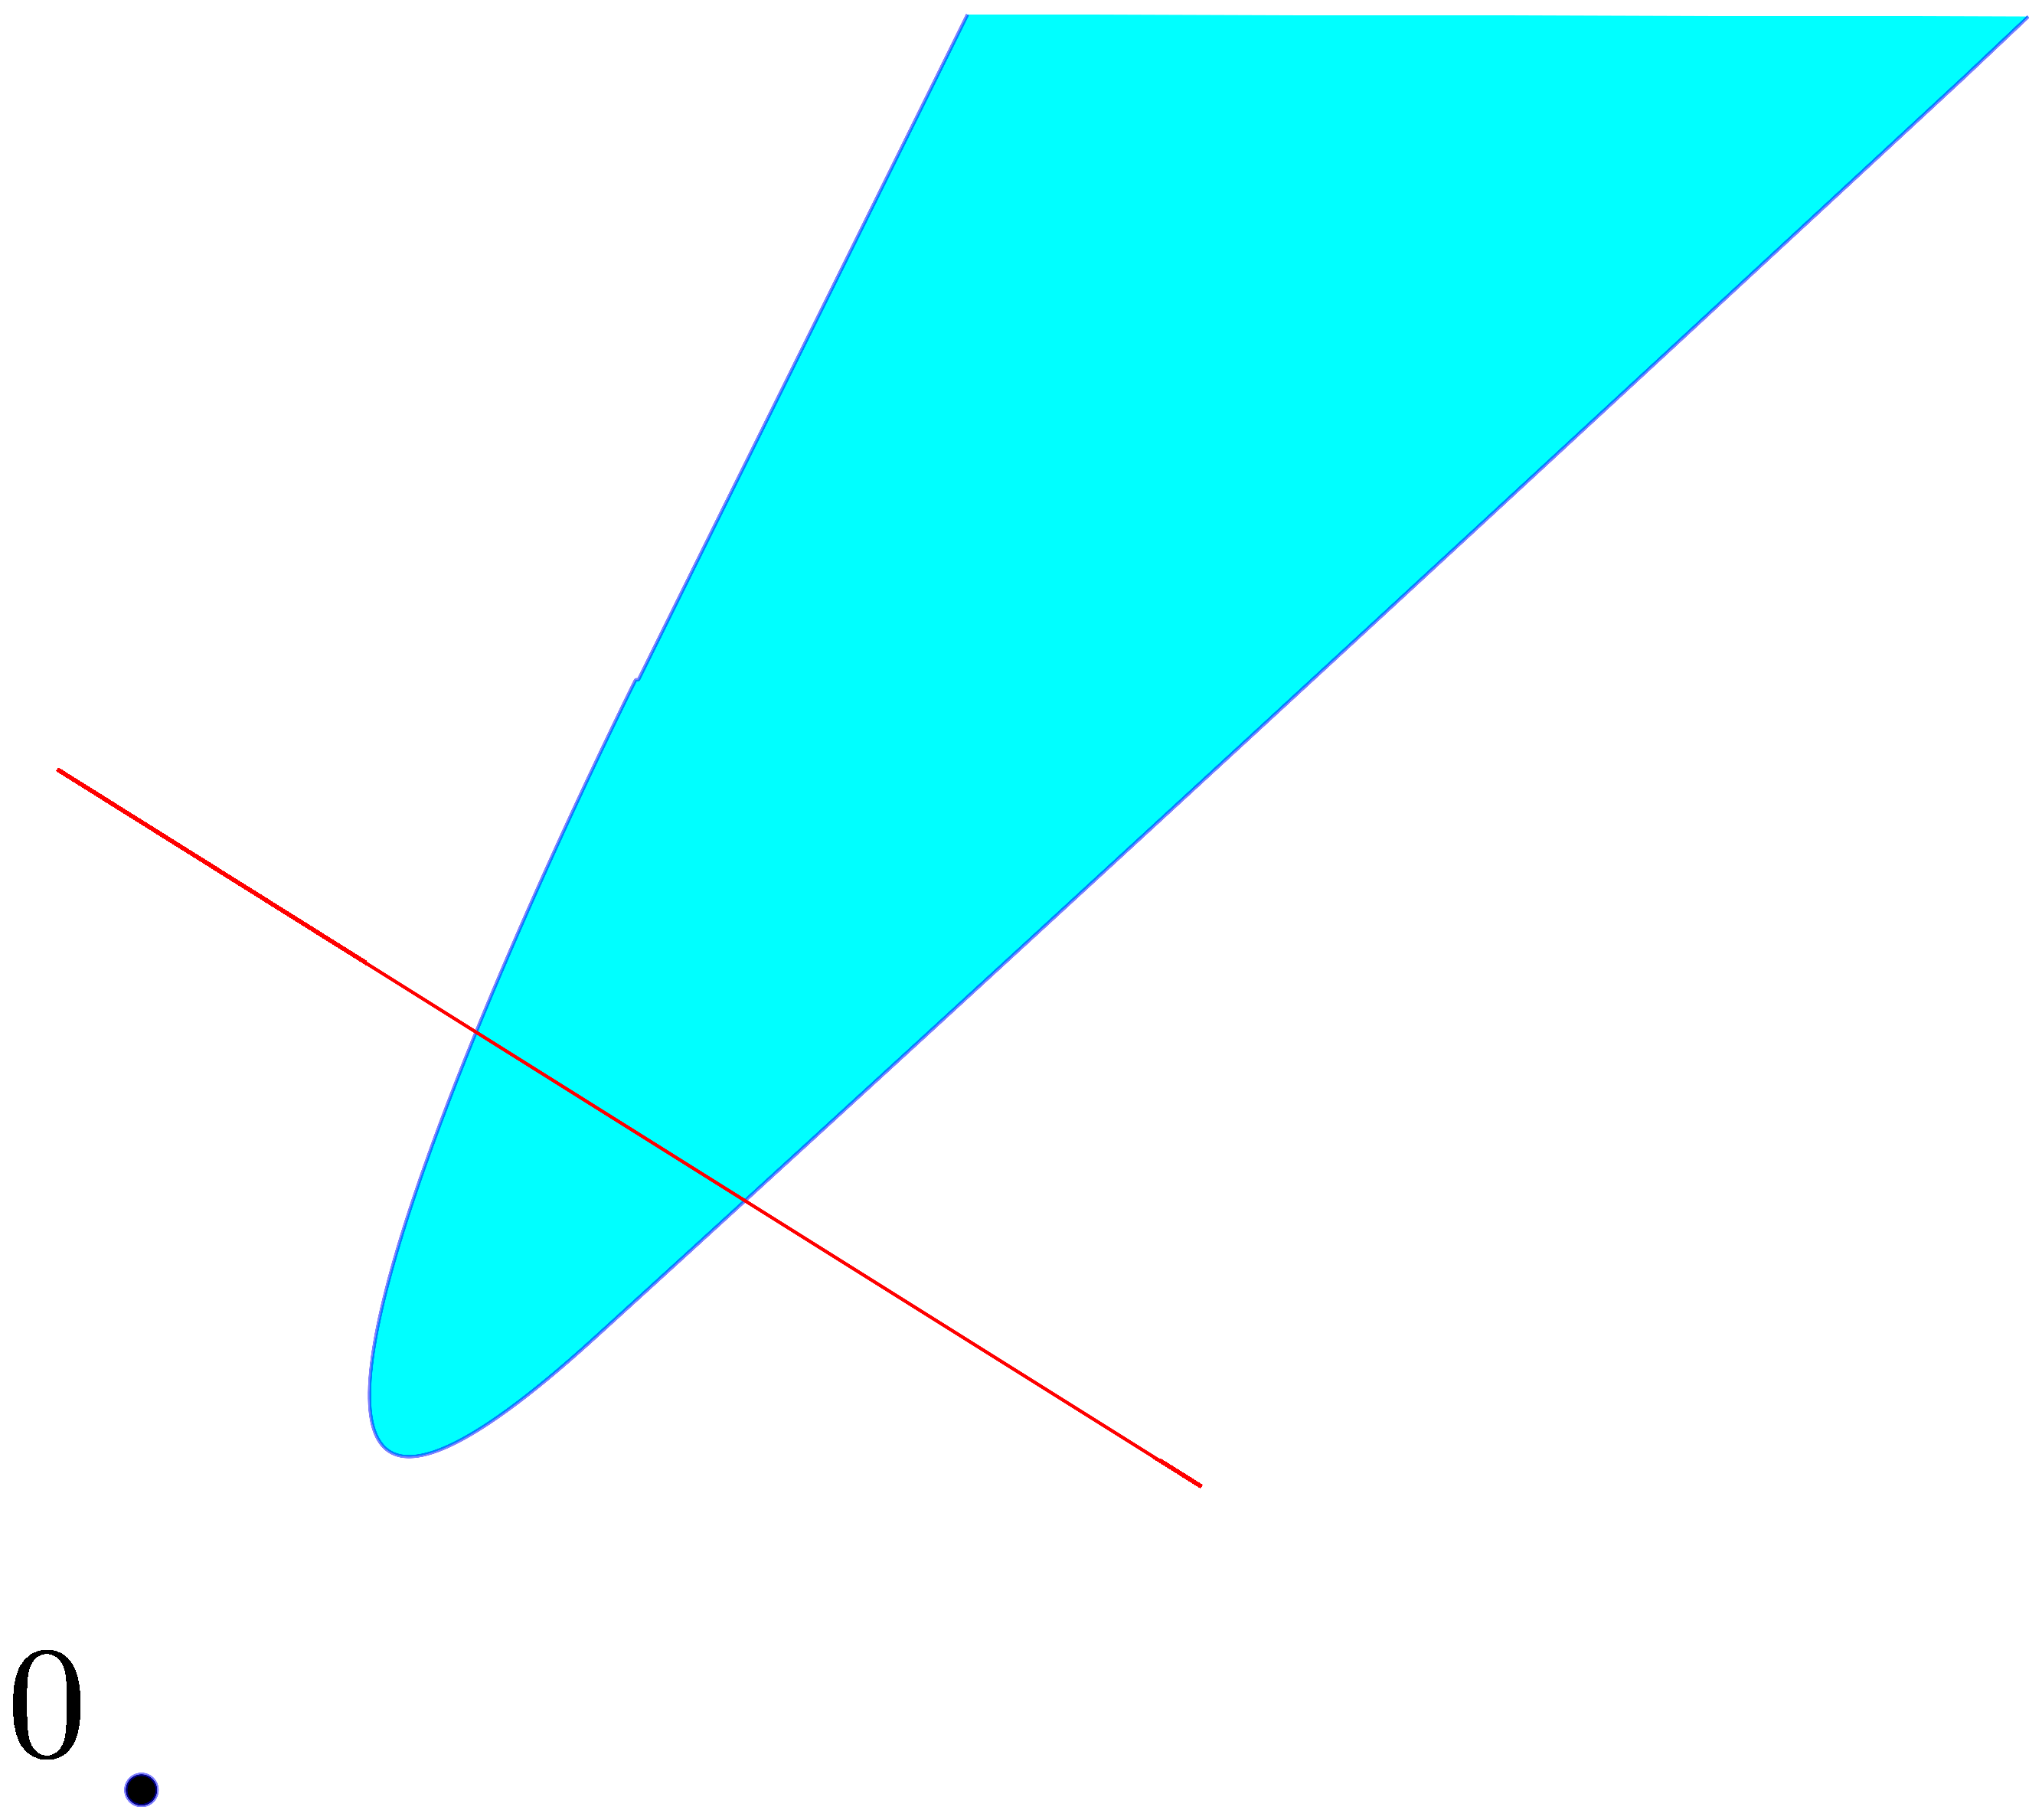
\includegraphics[keepaspectratio, scale=0.095]{figures/asymptotic_meaning_1.eps}
      \end{column}
      \pause
      \begin{column}{0.48\textwidth}
      \centering
      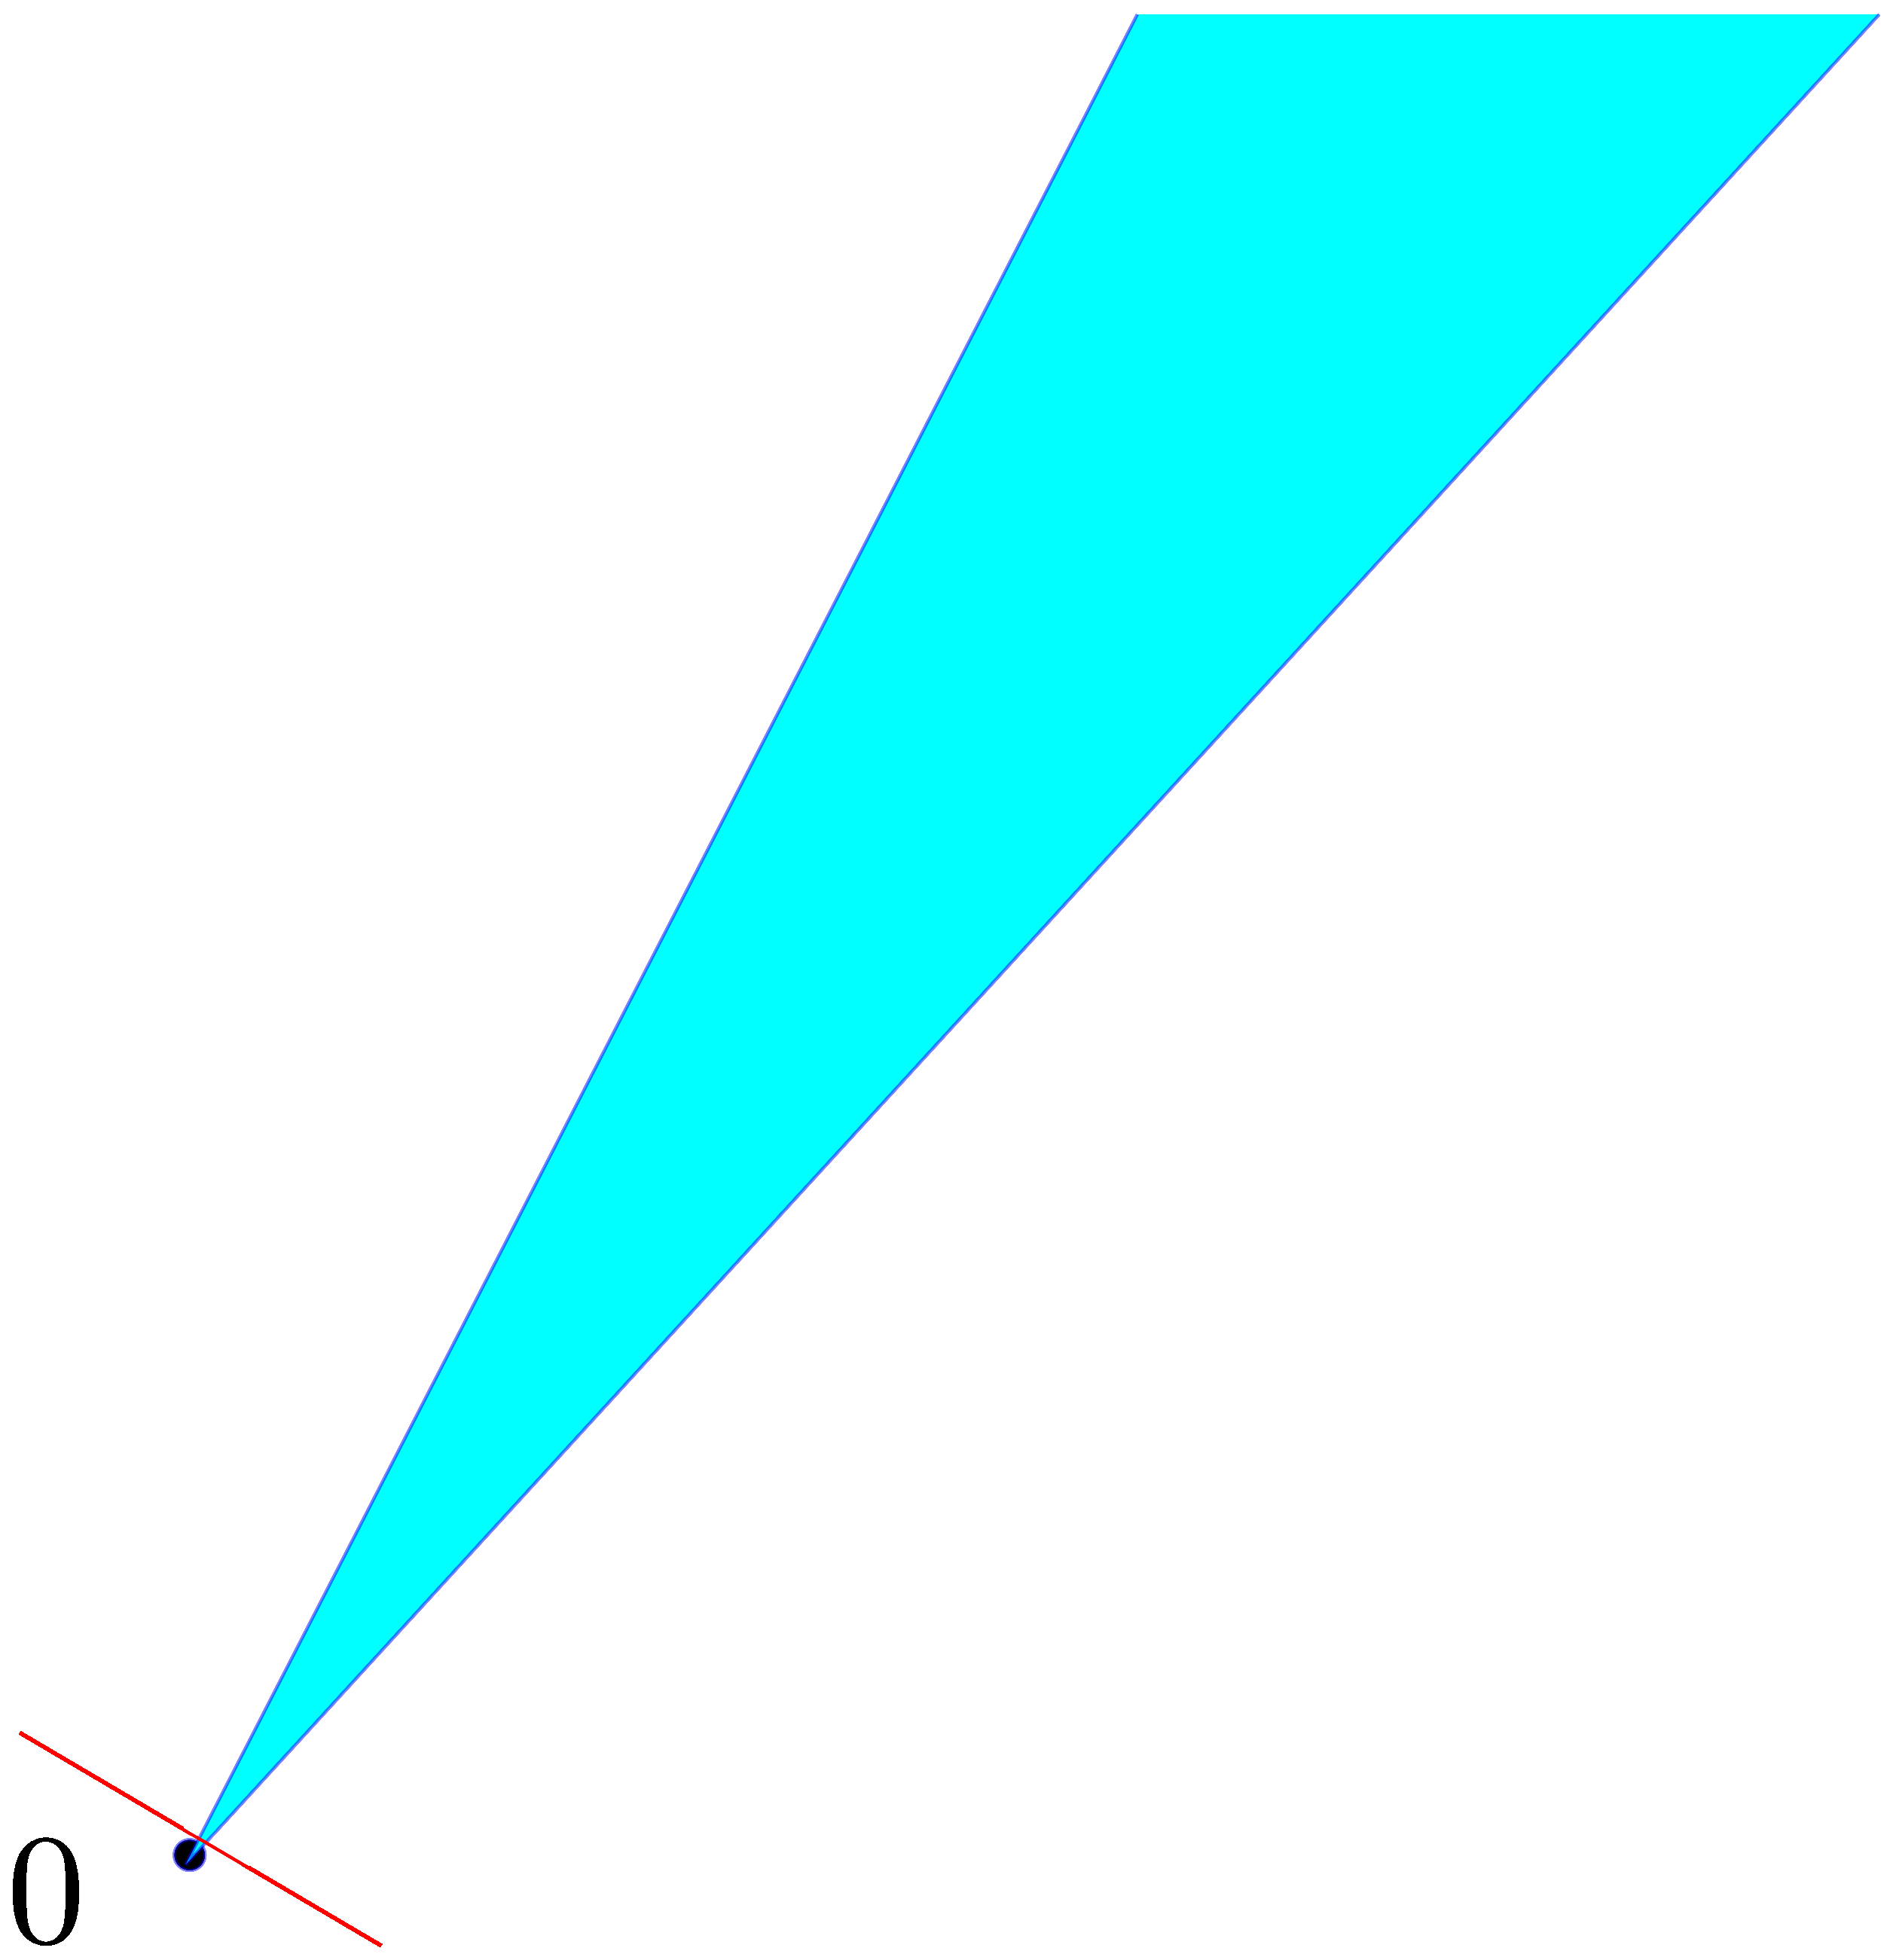
\includegraphics[keepaspectratio, scale=0.095]{figures/asymptotic_meaning_2.eps}
    \end{column}
  \end{columns}
\end{frame}

% 2.3
\begin{frame}{Definition of Asymptotic Cones}
  \begin{block}{Definition 1(Asymptotic Cones)}
    $C \subset \mathbb{R}^n$, $C \neq \emptyset$. Then, the asymptotic cone of the set $C$, denoted by $C_\infty$, is the set below with $\{ x_k \} \subset C$;
    \begin{equation}
      C_\infty = \left\{ d \in
      \mathbb{R}^n \:\middle|\: \exists t_k \rightarrow +\infty, \exists x_k \in C \:\text{with}\: \lim_{k \to \infty} \frac{x_k}{t_k} = d \right\}. \notag
    \end{equation}
  \end{block}

  Example: $C = \{(x,y) \in \mathbb{R}^2 \:|\: y=x^2\}$. We let $\textcolor{blue}{x_k} = (k, k^2)$ and $t_k = \left\lVert x_k \right\rVert$.

  \centering
  \begin{columns}
    \pause
    \begin{column}{0.48\textwidth}
    \centering
    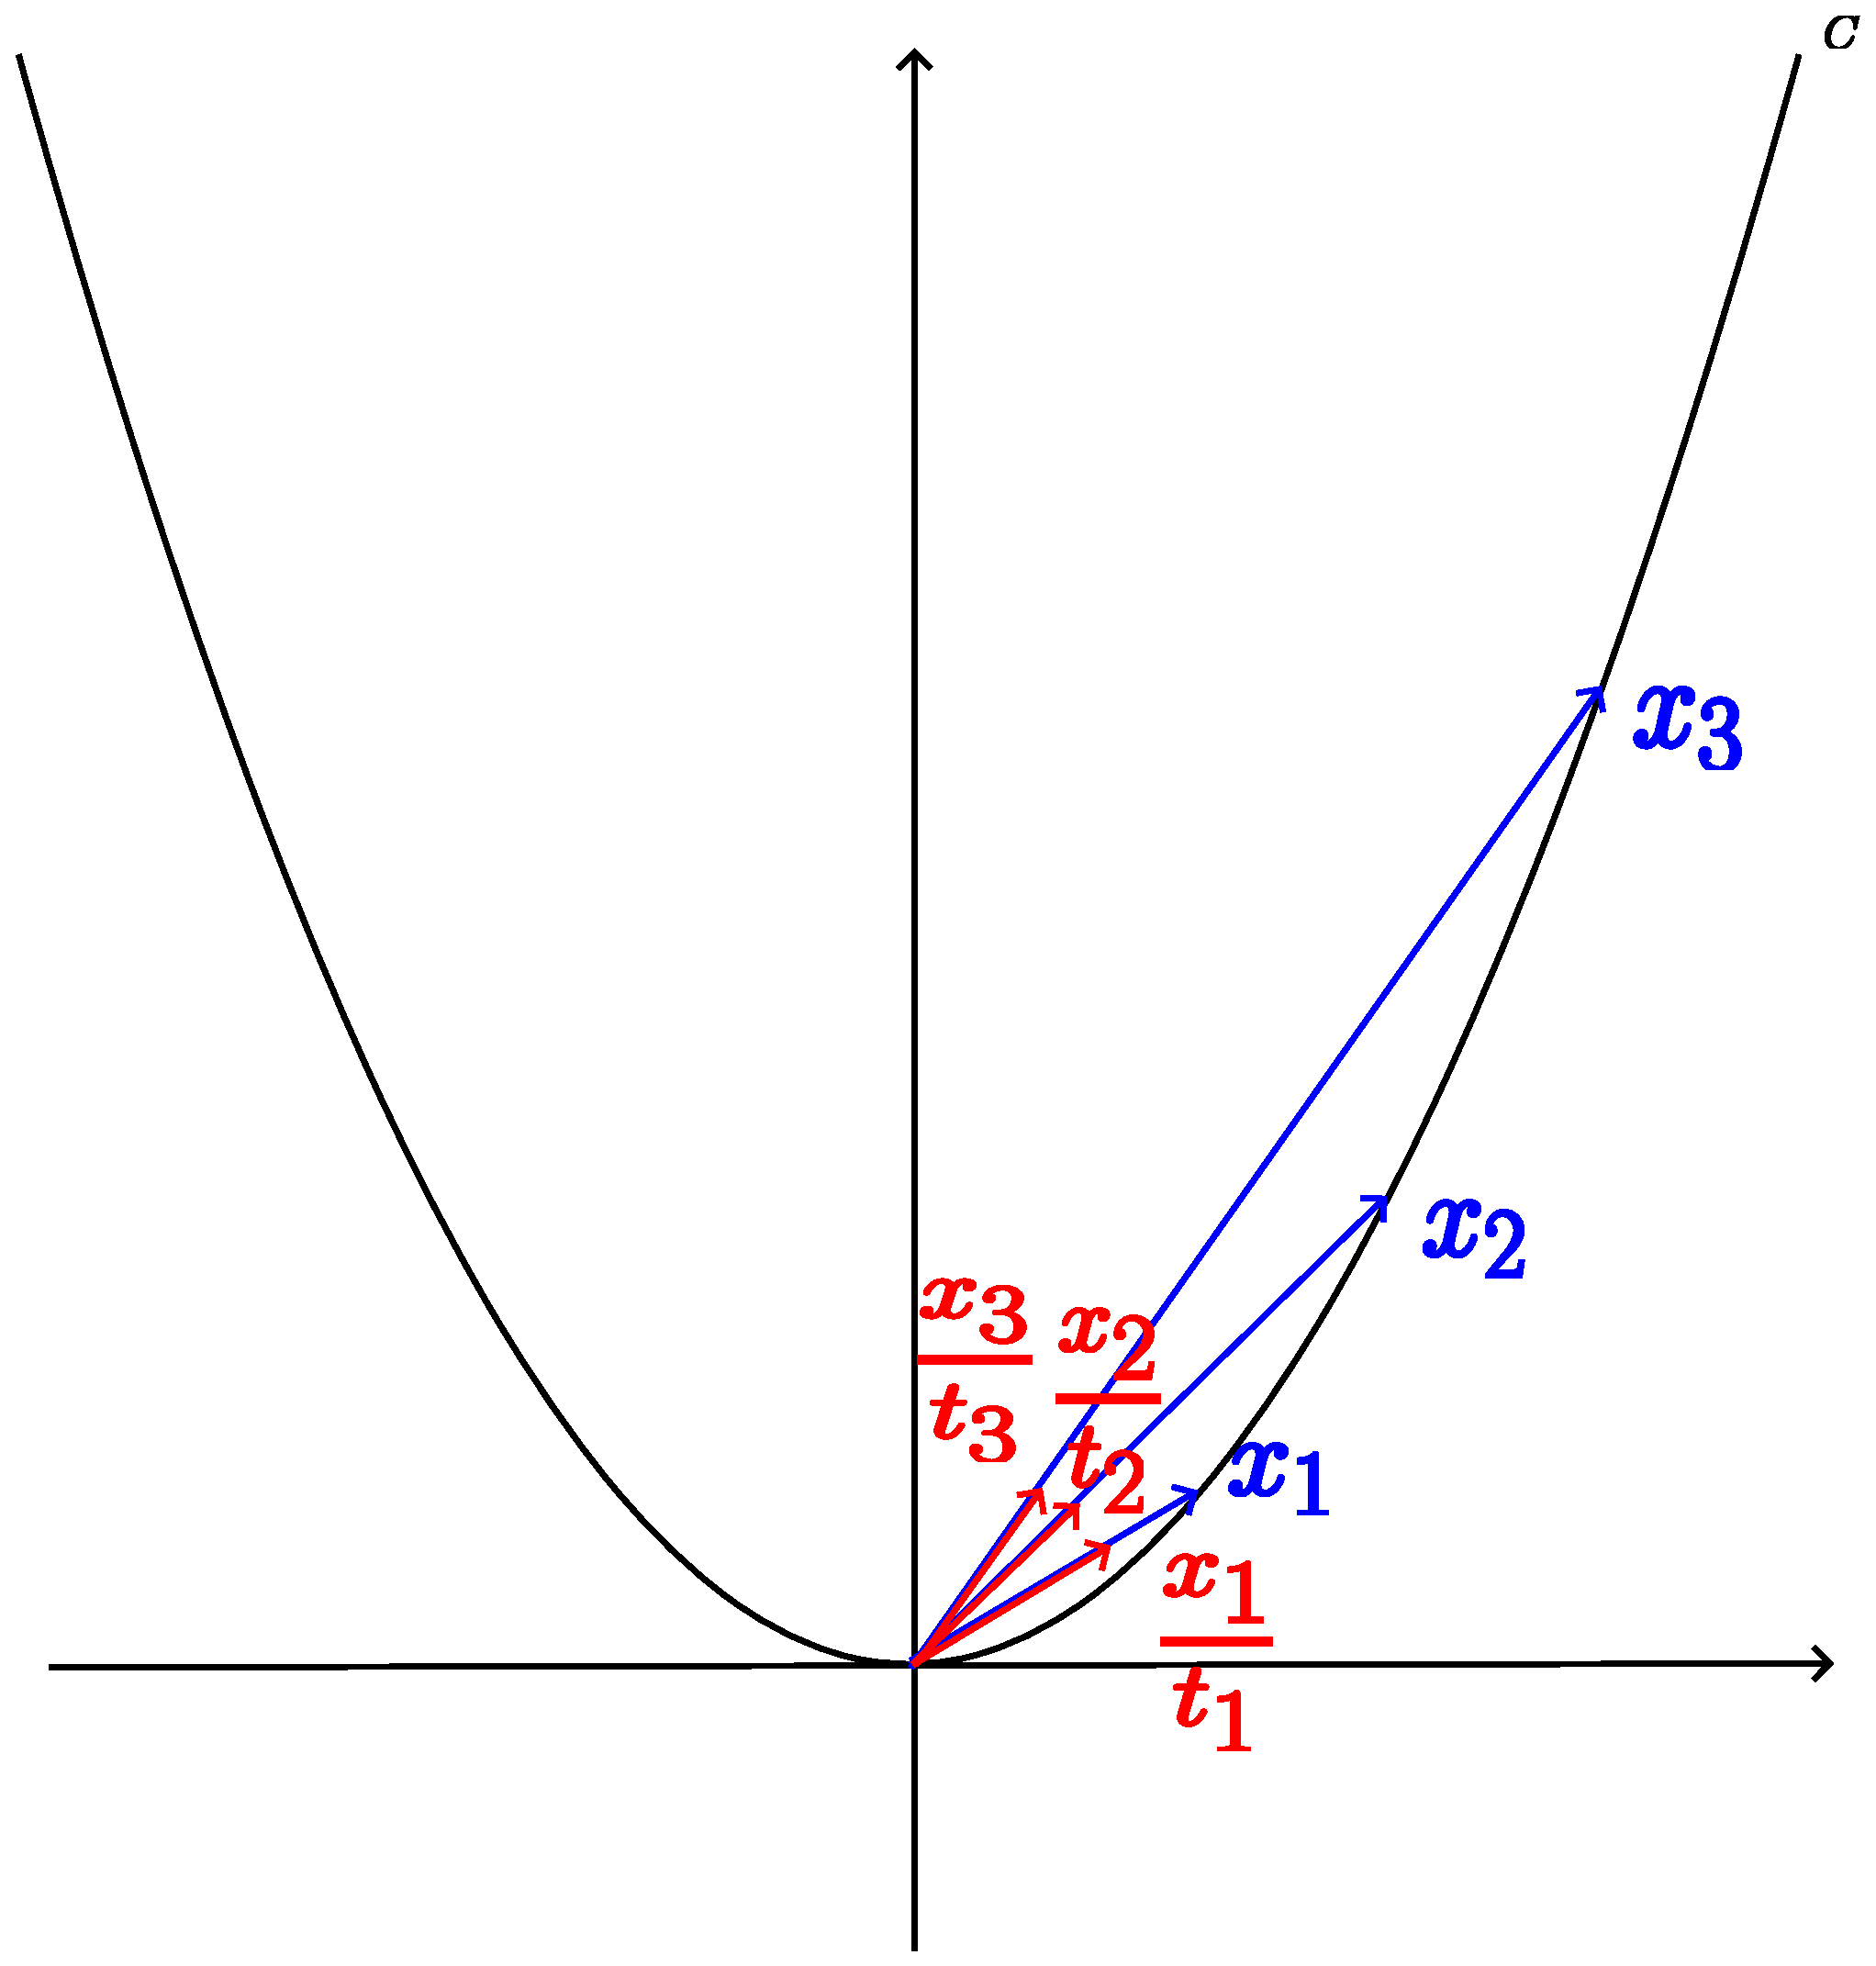
\includegraphics[keepaspectratio, scale=0.09]{figures/figure_asymptotic_cone_1.eps}
    \end{column}
    \pause
    \begin{column}{0.48\textwidth}
    \centering
    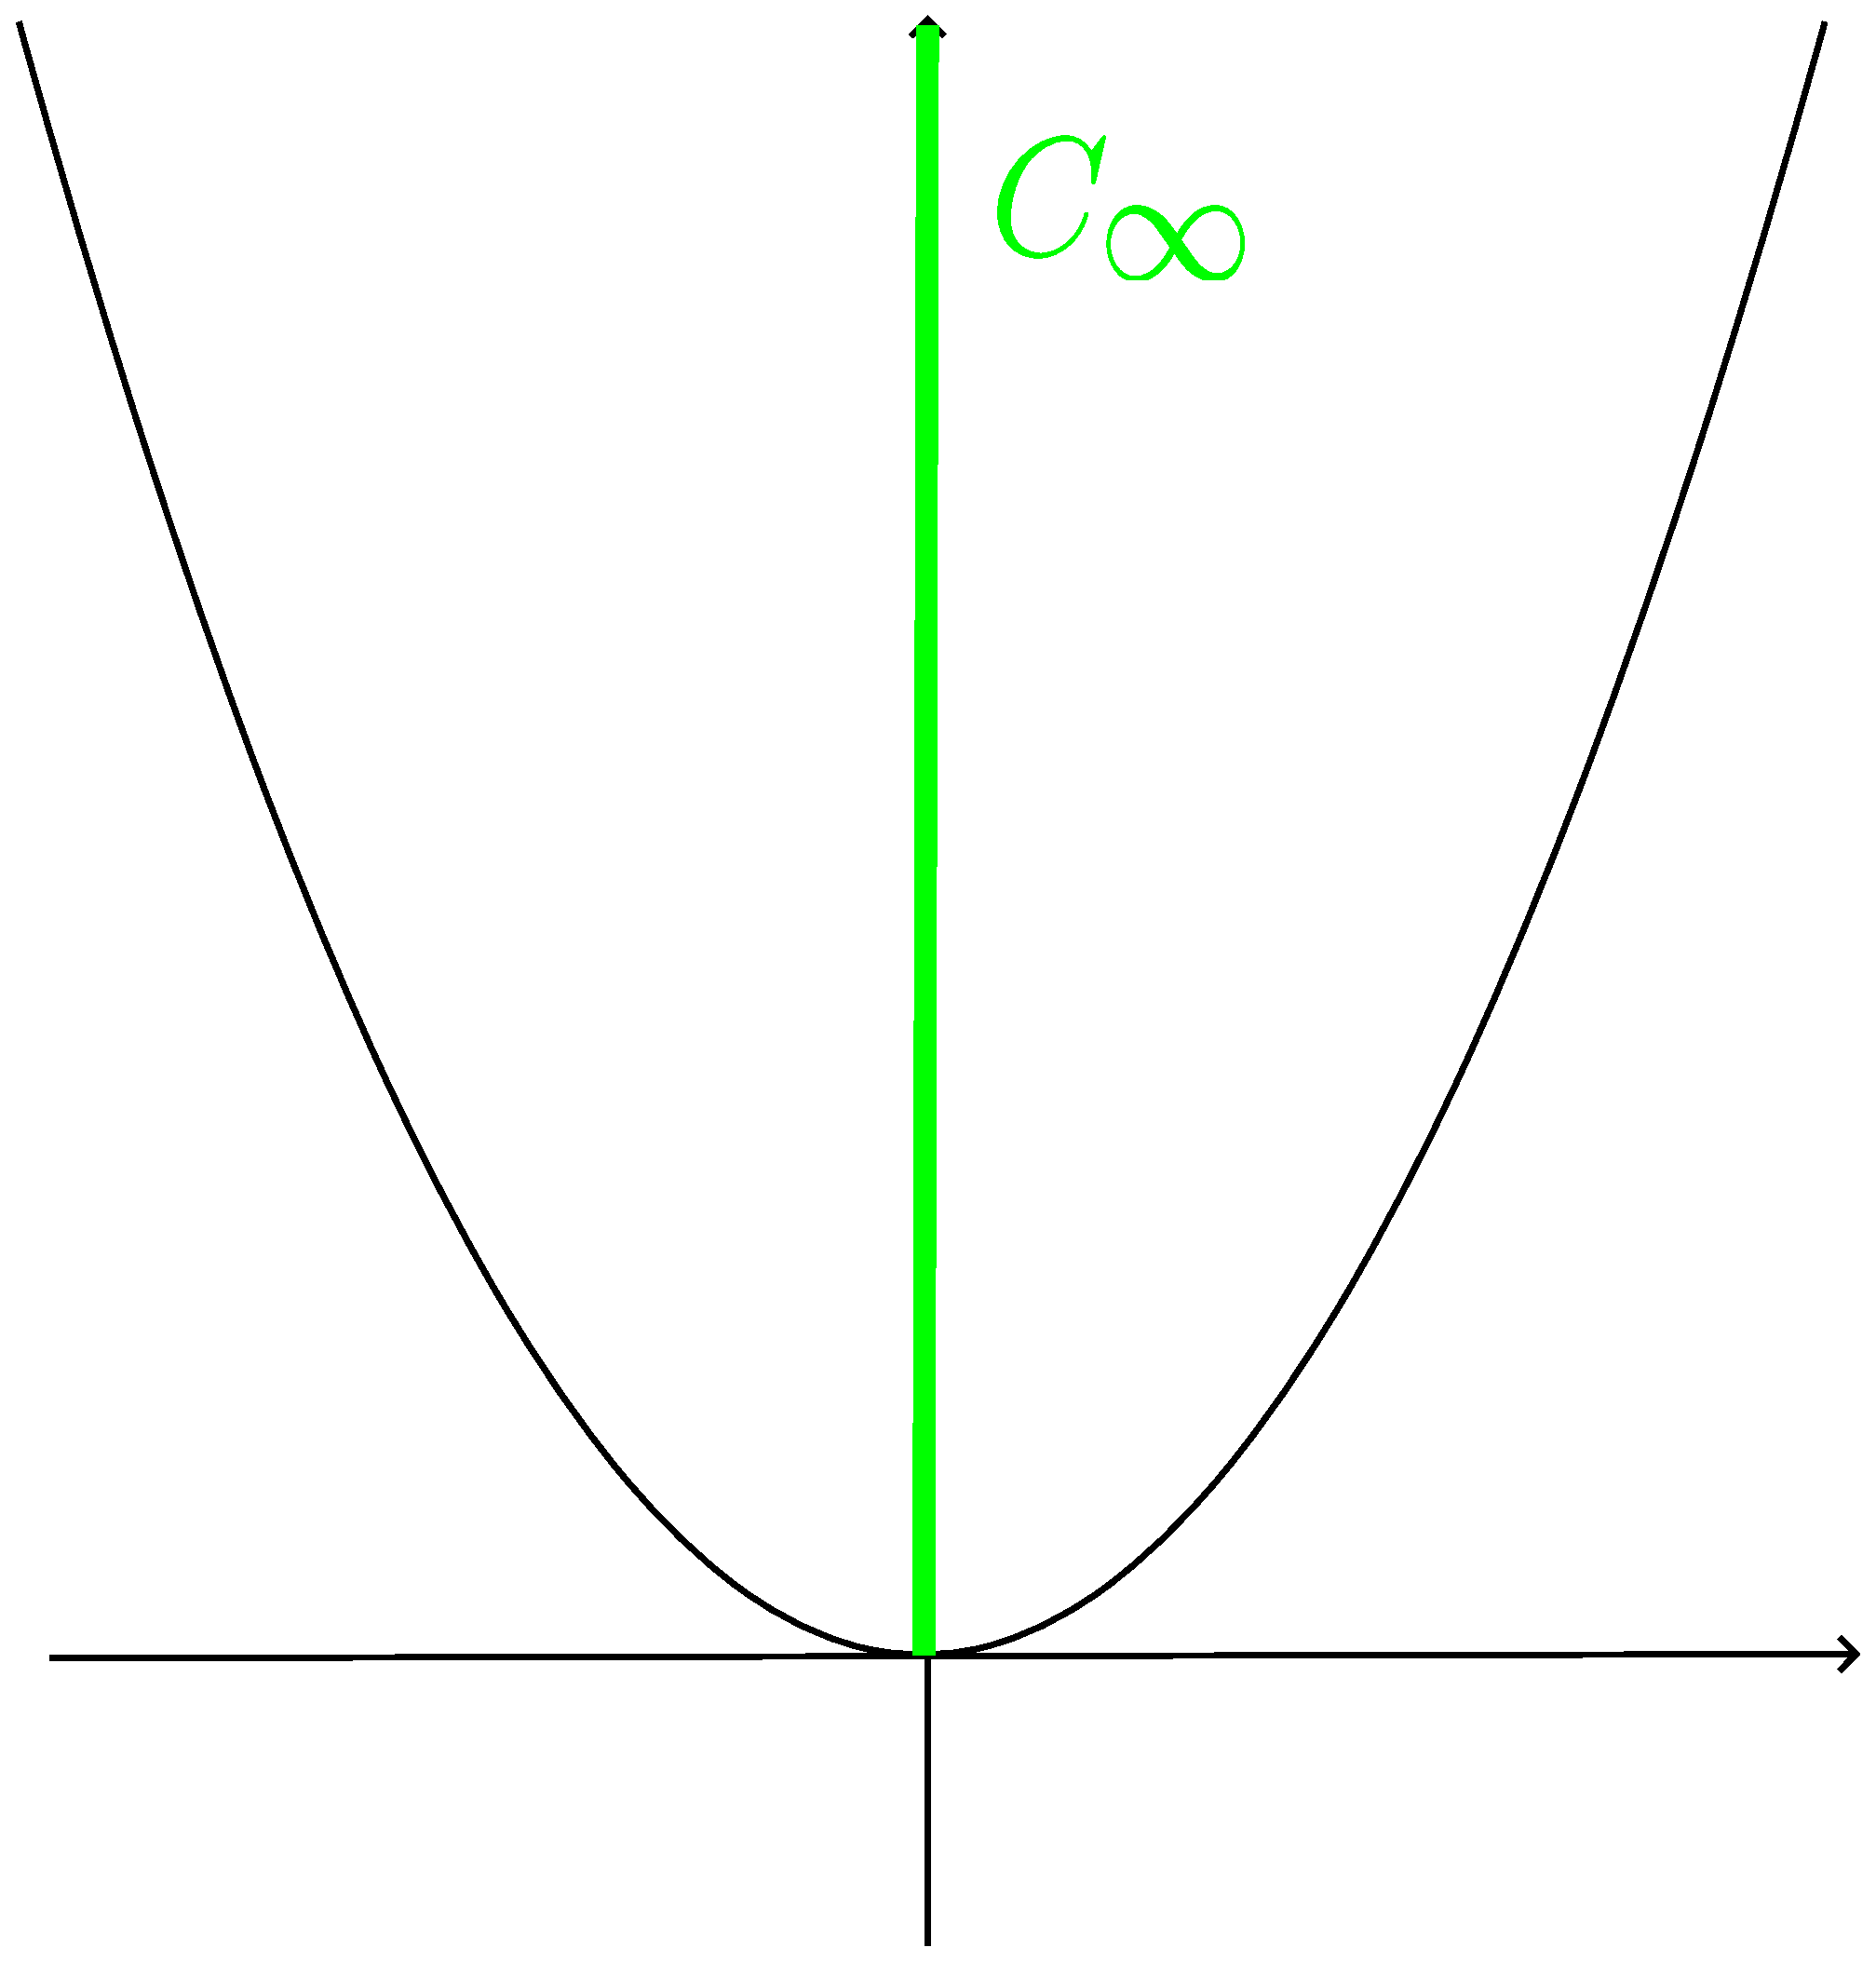
\includegraphics[keepaspectratio, scale=0.09]{figures/figure_asymptotic_cone_2.eps}
    \end{column}
  \end{columns}
\end{frame}


% 2.4
\begin{frame}{Properties around Asymptotic Cones}
  \begin{block}{Proposition 1}
    A set $C \subset \mathbb{R}^n$ is bounded if and only if $C_\infty = \{0\}$.
  \end{block}

  \begin{block}{Definition 2}
    Let $C \subset \NDemenstionalRealEuclidianSpace$ be nonempty and define
    \begin{equation}
      C_{\infty}^1 = \left\{d \in \NDemenstionalRealEuclidianSpace \:\middle|\: \forall t_k \rightarrow + \infty , \exists x_k \in C \:\text{ with }\: \lim_{k \to \infty} \frac{x_k}{t_k} = d \right\}. \notag
    \end{equation}
    We say that $C$ is asymptotically regular if $C_{\infty} = C_{\infty}^1$.
  \end{block}

  \begin{block}{Proposition 2}
    Let $C$ be a nonempty convex set in $\NDemenstionalRealEuclidianSpace$. Then $C$ is asymptotically regular.
  \end{block}
\end{frame}

% 2.5
\begin{frame}{Example of Asymptotically Regular}
  \begin{block}{Definition 2}
    Let $C \subset \NDemenstionalRealEuclidianSpace$ be nonempty and define
    \begin{equation}
      C_{\infty}^1 = \left\{d \in \NDemenstionalRealEuclidianSpace \:\middle|\: \forall t_k \rightarrow + \infty , \exists x_k \in C \:\text{ with }\: \lim_{k \to \infty} \frac{x_k}{t_k} = d \right\}. \notag
    \end{equation}
    We say that $C$ is asymptotically regular if $C_{\infty} = C_{\infty}^1$.
  \end{block}

  Example: $D$ is NOT asymptotically regular.

  \centering
  \begin{columns}
    \begin{column}{0.48\textwidth}
    \centering
    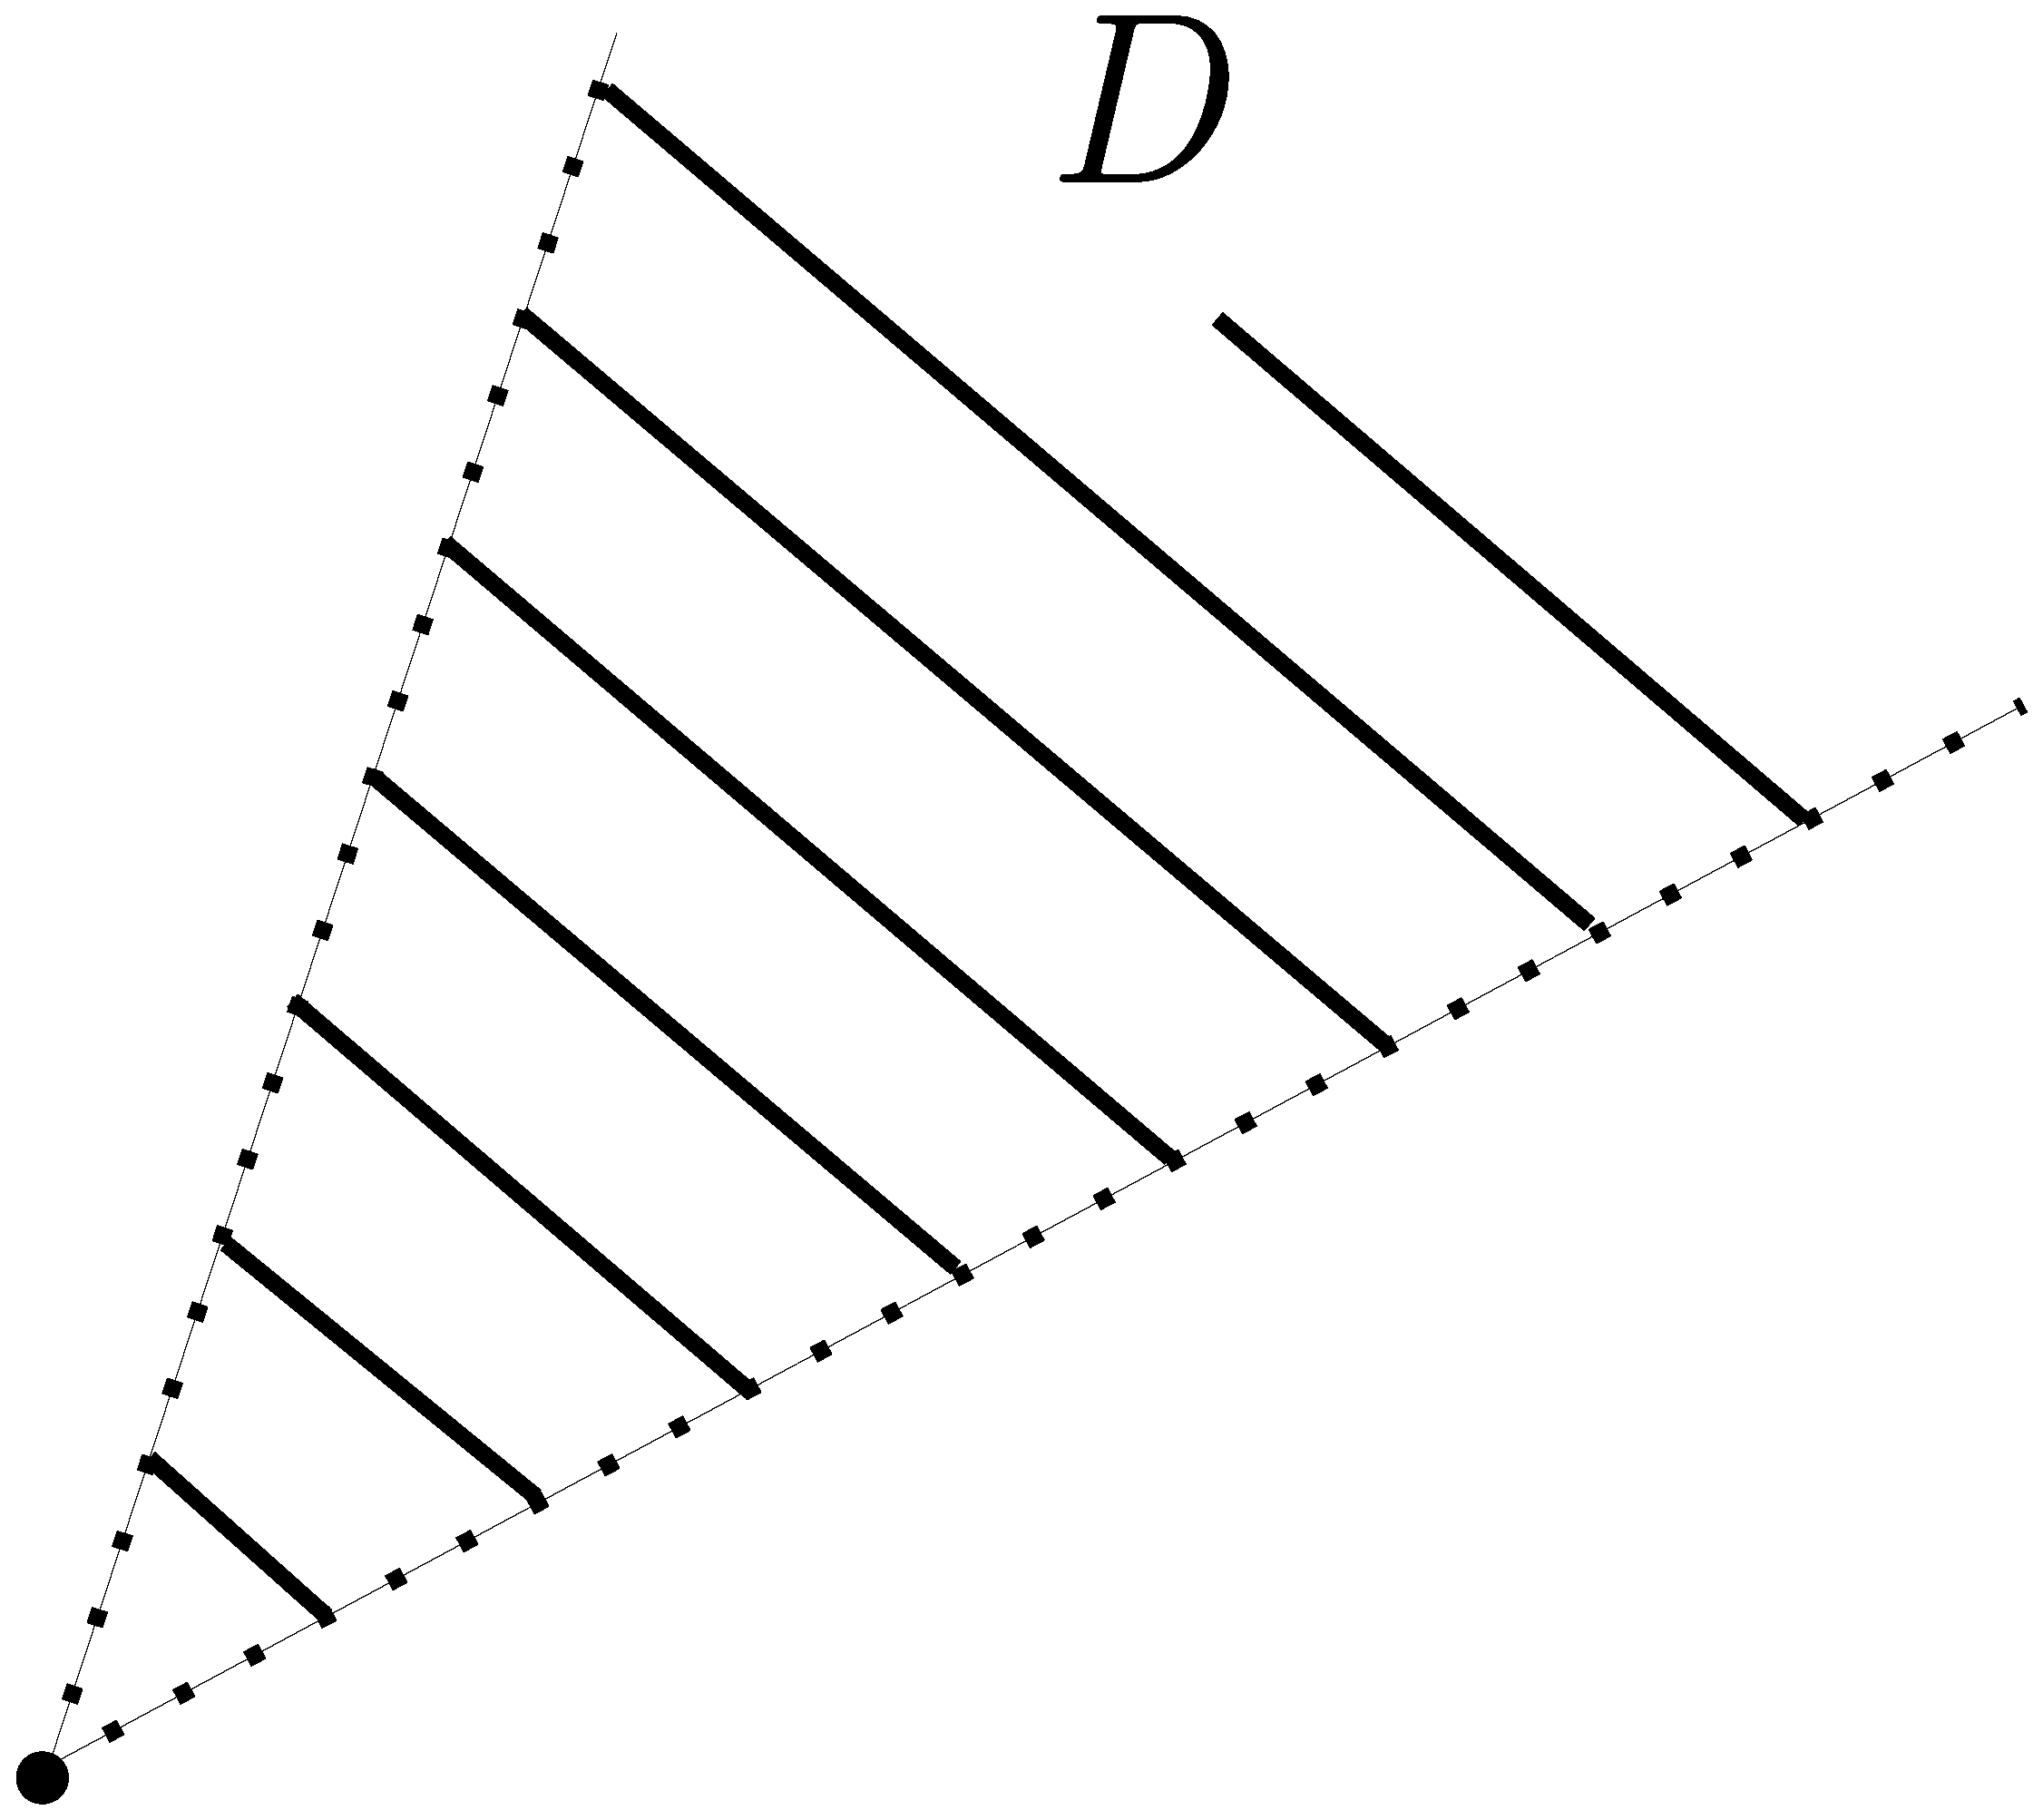
\includegraphics[keepaspectratio, scale=0.085]{figures/example_not_asymptotically_regular_1.eps}
    \end{column}
    \pause
    \begin{column}{0.48\textwidth}
    \centering
    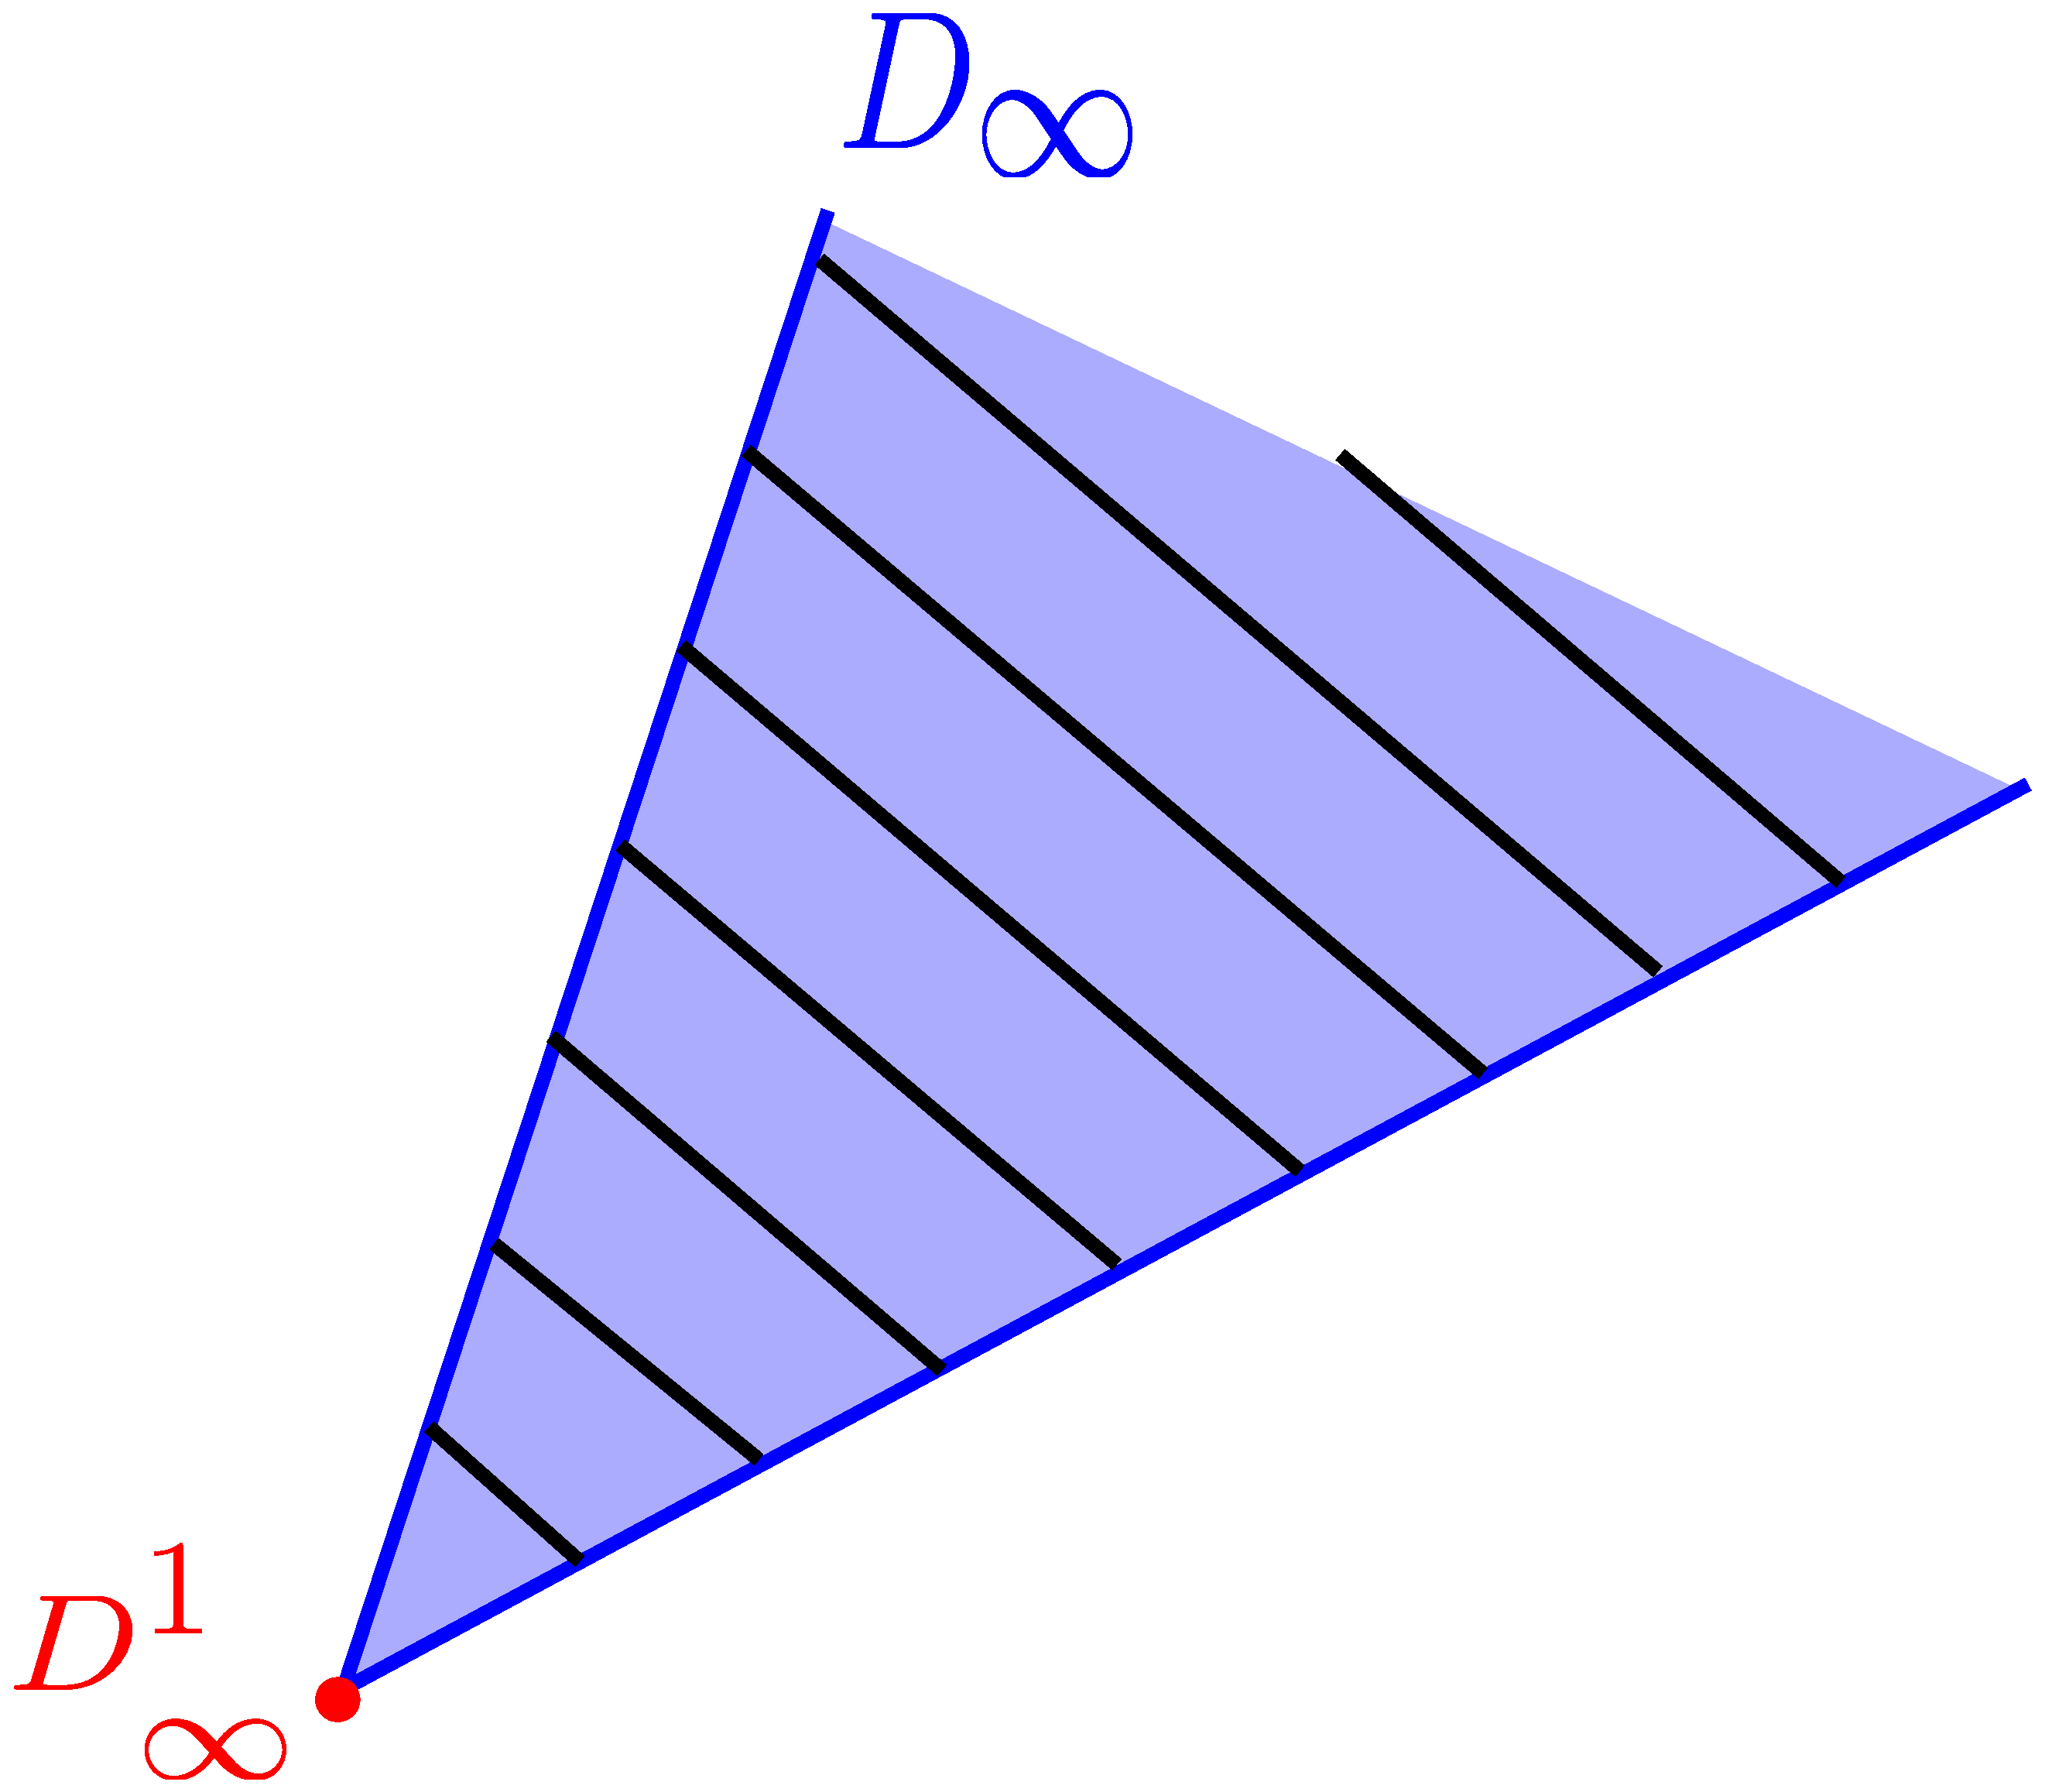
\includegraphics[keepaspectratio, scale=0.085]{figures/example_not_asymptotically_regular_2.eps}
    \end{column}
  \end{columns}
\end{frame}

% 2.6
\begin{frame}{Example of Asymptotically Regular}
  \begin{block}{Proposition 2}
    Let $C$ be a nonempty convex set in $\NDemenstionalRealEuclidianSpace$. Then $C$ is asymptotically regular.
  \end{block}

  Example: $E$ is not convex but $E$ is asymptotically regular.

  \medskip

  \centering
  \begin{columns}
    \begin{column}{0.48\textwidth}
    \centering
    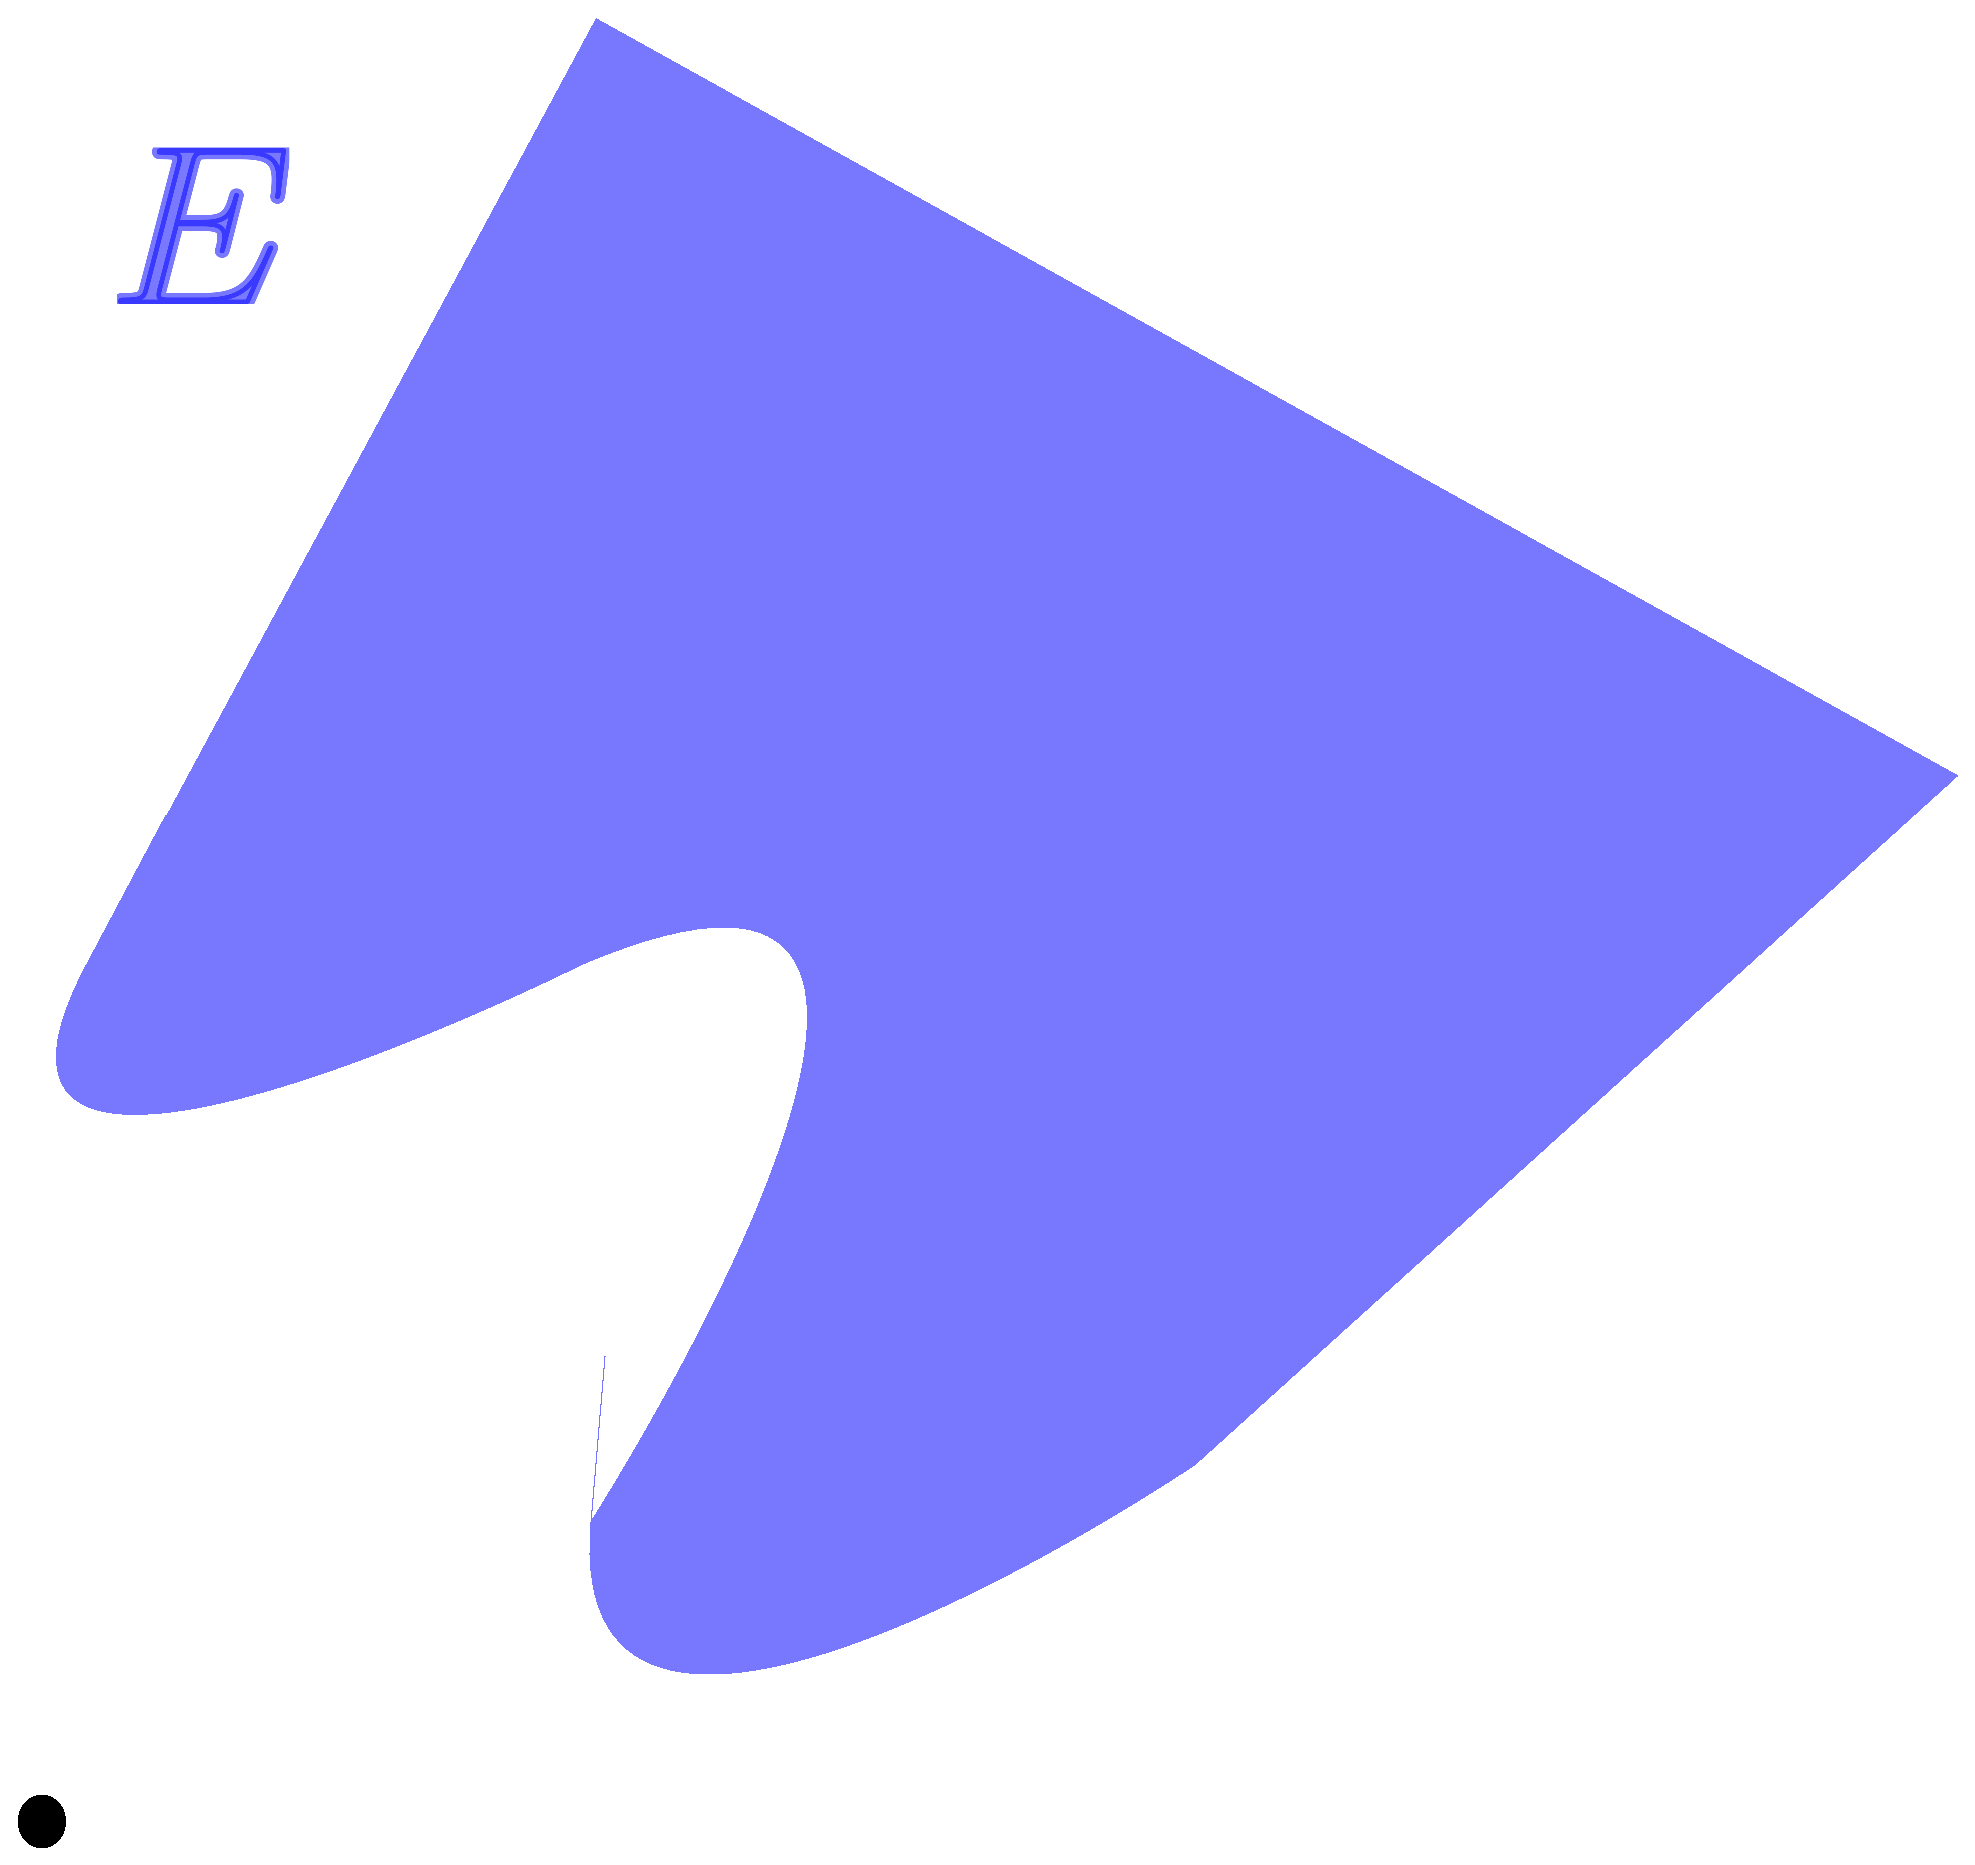
\includegraphics[keepaspectratio, scale=0.095]{figures/example_not_convex_asymptotically_regular_1.eps}
    \end{column}
    \pause
    \begin{column}{0.48\textwidth}
    \centering
    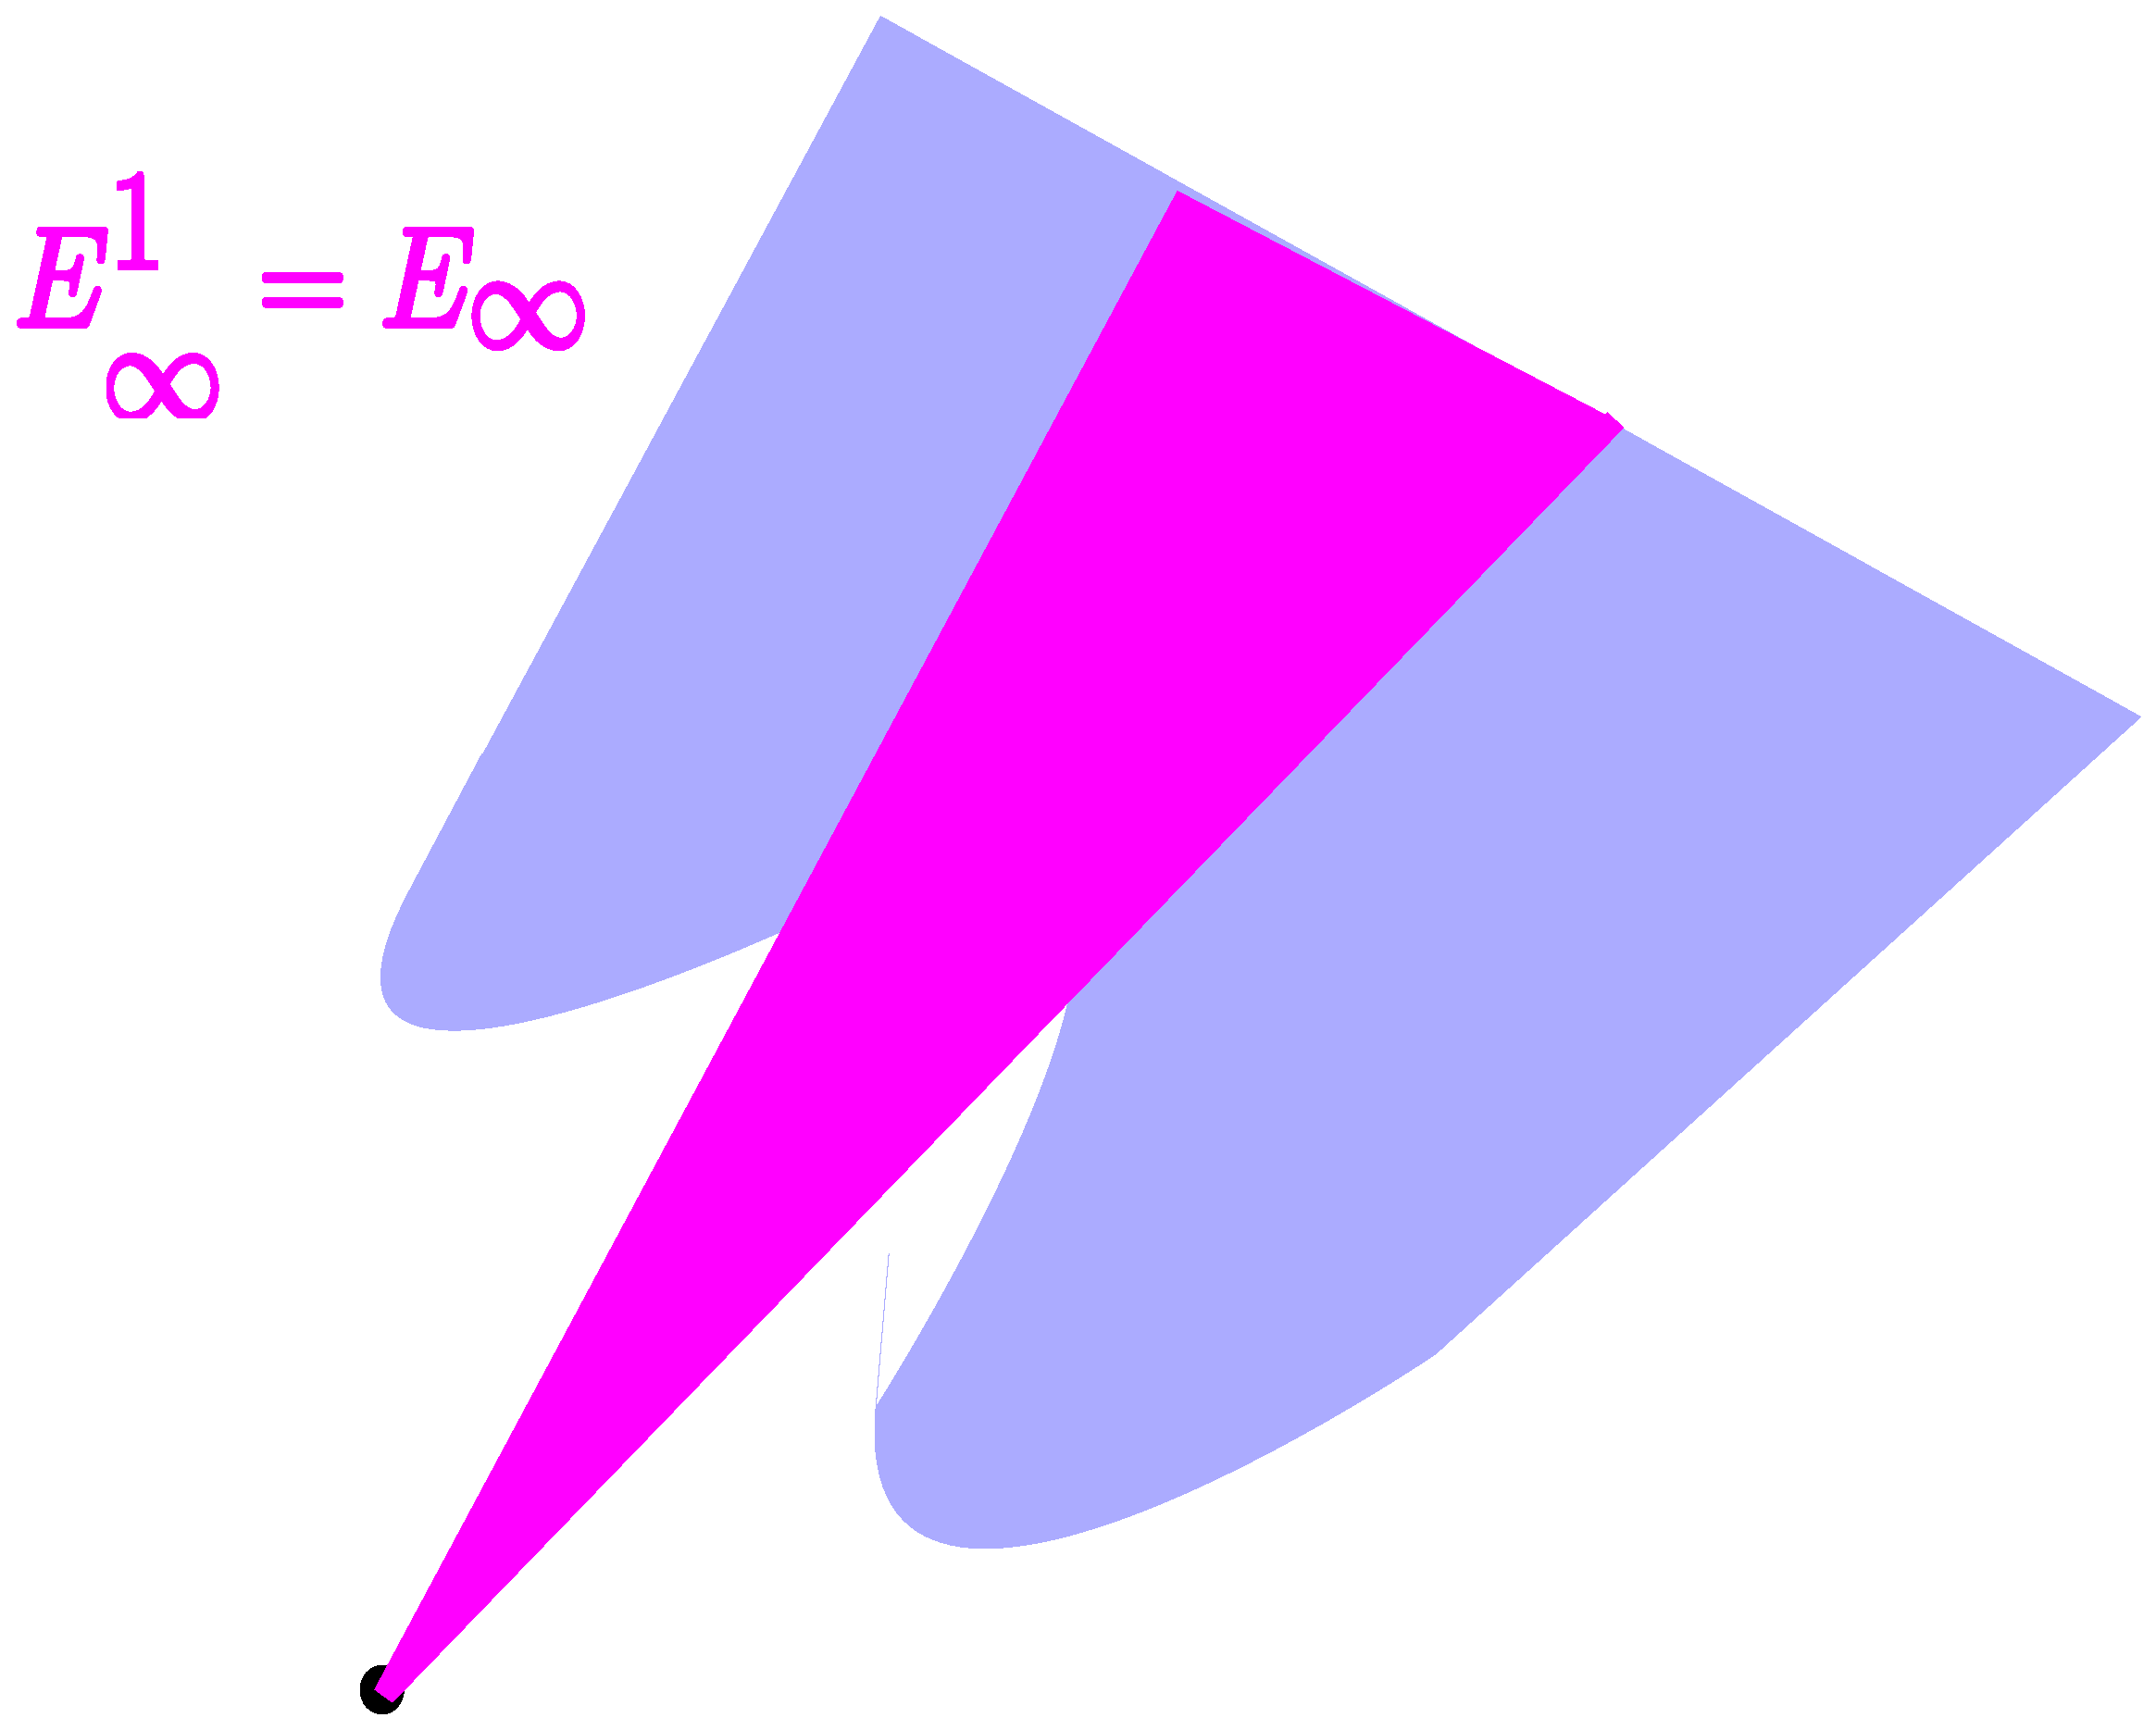
\includegraphics[keepaspectratio, scale=0.095]{figures/example_not_convex_asymptotically_regular_2.eps}
    \end{column}
  \end{columns}
\end{frame}

% 3.Painleve-Kuratowski Convergence
% ----------------------------------------------------------------
\section{\Painleve-Kuratowski Convergence}
\begin{frame}{Contents}
  \tableofcontents[currentsection]
\end{frame}

% 3.1
\begin{frame}{Definition of the \Painleve-Kuratowski Convergence}
  \begin{block}{Definition 3}
    $Y$: a topological vector space.

    $\mathcal{P}(Y)$: a family of subset in $Y$.

    Let $(A_n)_{n \in \NaturalNumberSet} \subset \mathcal{P}(Y)$. We define the inner limit and the outer limit as

    \begin{equation}
      \begin{split}
        \liminf_{n \to \infty}A_n &\coloneqq \SetForm{y \in Y}{\exists (y_n) \to y \SuchThat y_n \in A_n \:\text{for}\: n \geq n_0}, \\
        \limsup_{n \to \infty}A_n &\coloneqq \SetForm{y \in Y}{\exists (y_{n(k)}) \to y \SuchThat y_{n(k)} \in A_{n(k)} \:\text{for}\: k \in \NaturalNumberSet}. \notag
      \end{split}
    \end{equation}

    If it holds that $\liminf_{n \to \infty}A_n \supset \limsup_{n \to \infty}A_n$, we say that $(A_n)$ converges in the sense of \Painleve-Kuratowski.
  \end{block}
\end{frame}

% 3.2
\begin{frame}[t]{\Painleve-Kuratowski Convergence Examples}
  Example:

  \centering
  \begin{columns}
    \begin{column}{0.48\textwidth}
    \centering
    \begin{equation}
      A_n = \begin{cases} [0, 1],  & \mbox{if }n\mbox{ is odd} \\ [0, \frac{1}{n}], & \mbox{if }n\mbox{ is even} \end{cases} \notag
    \end{equation}
    \end{column}
    \pause
    \begin{column}{0.48\textwidth}
    \centering
    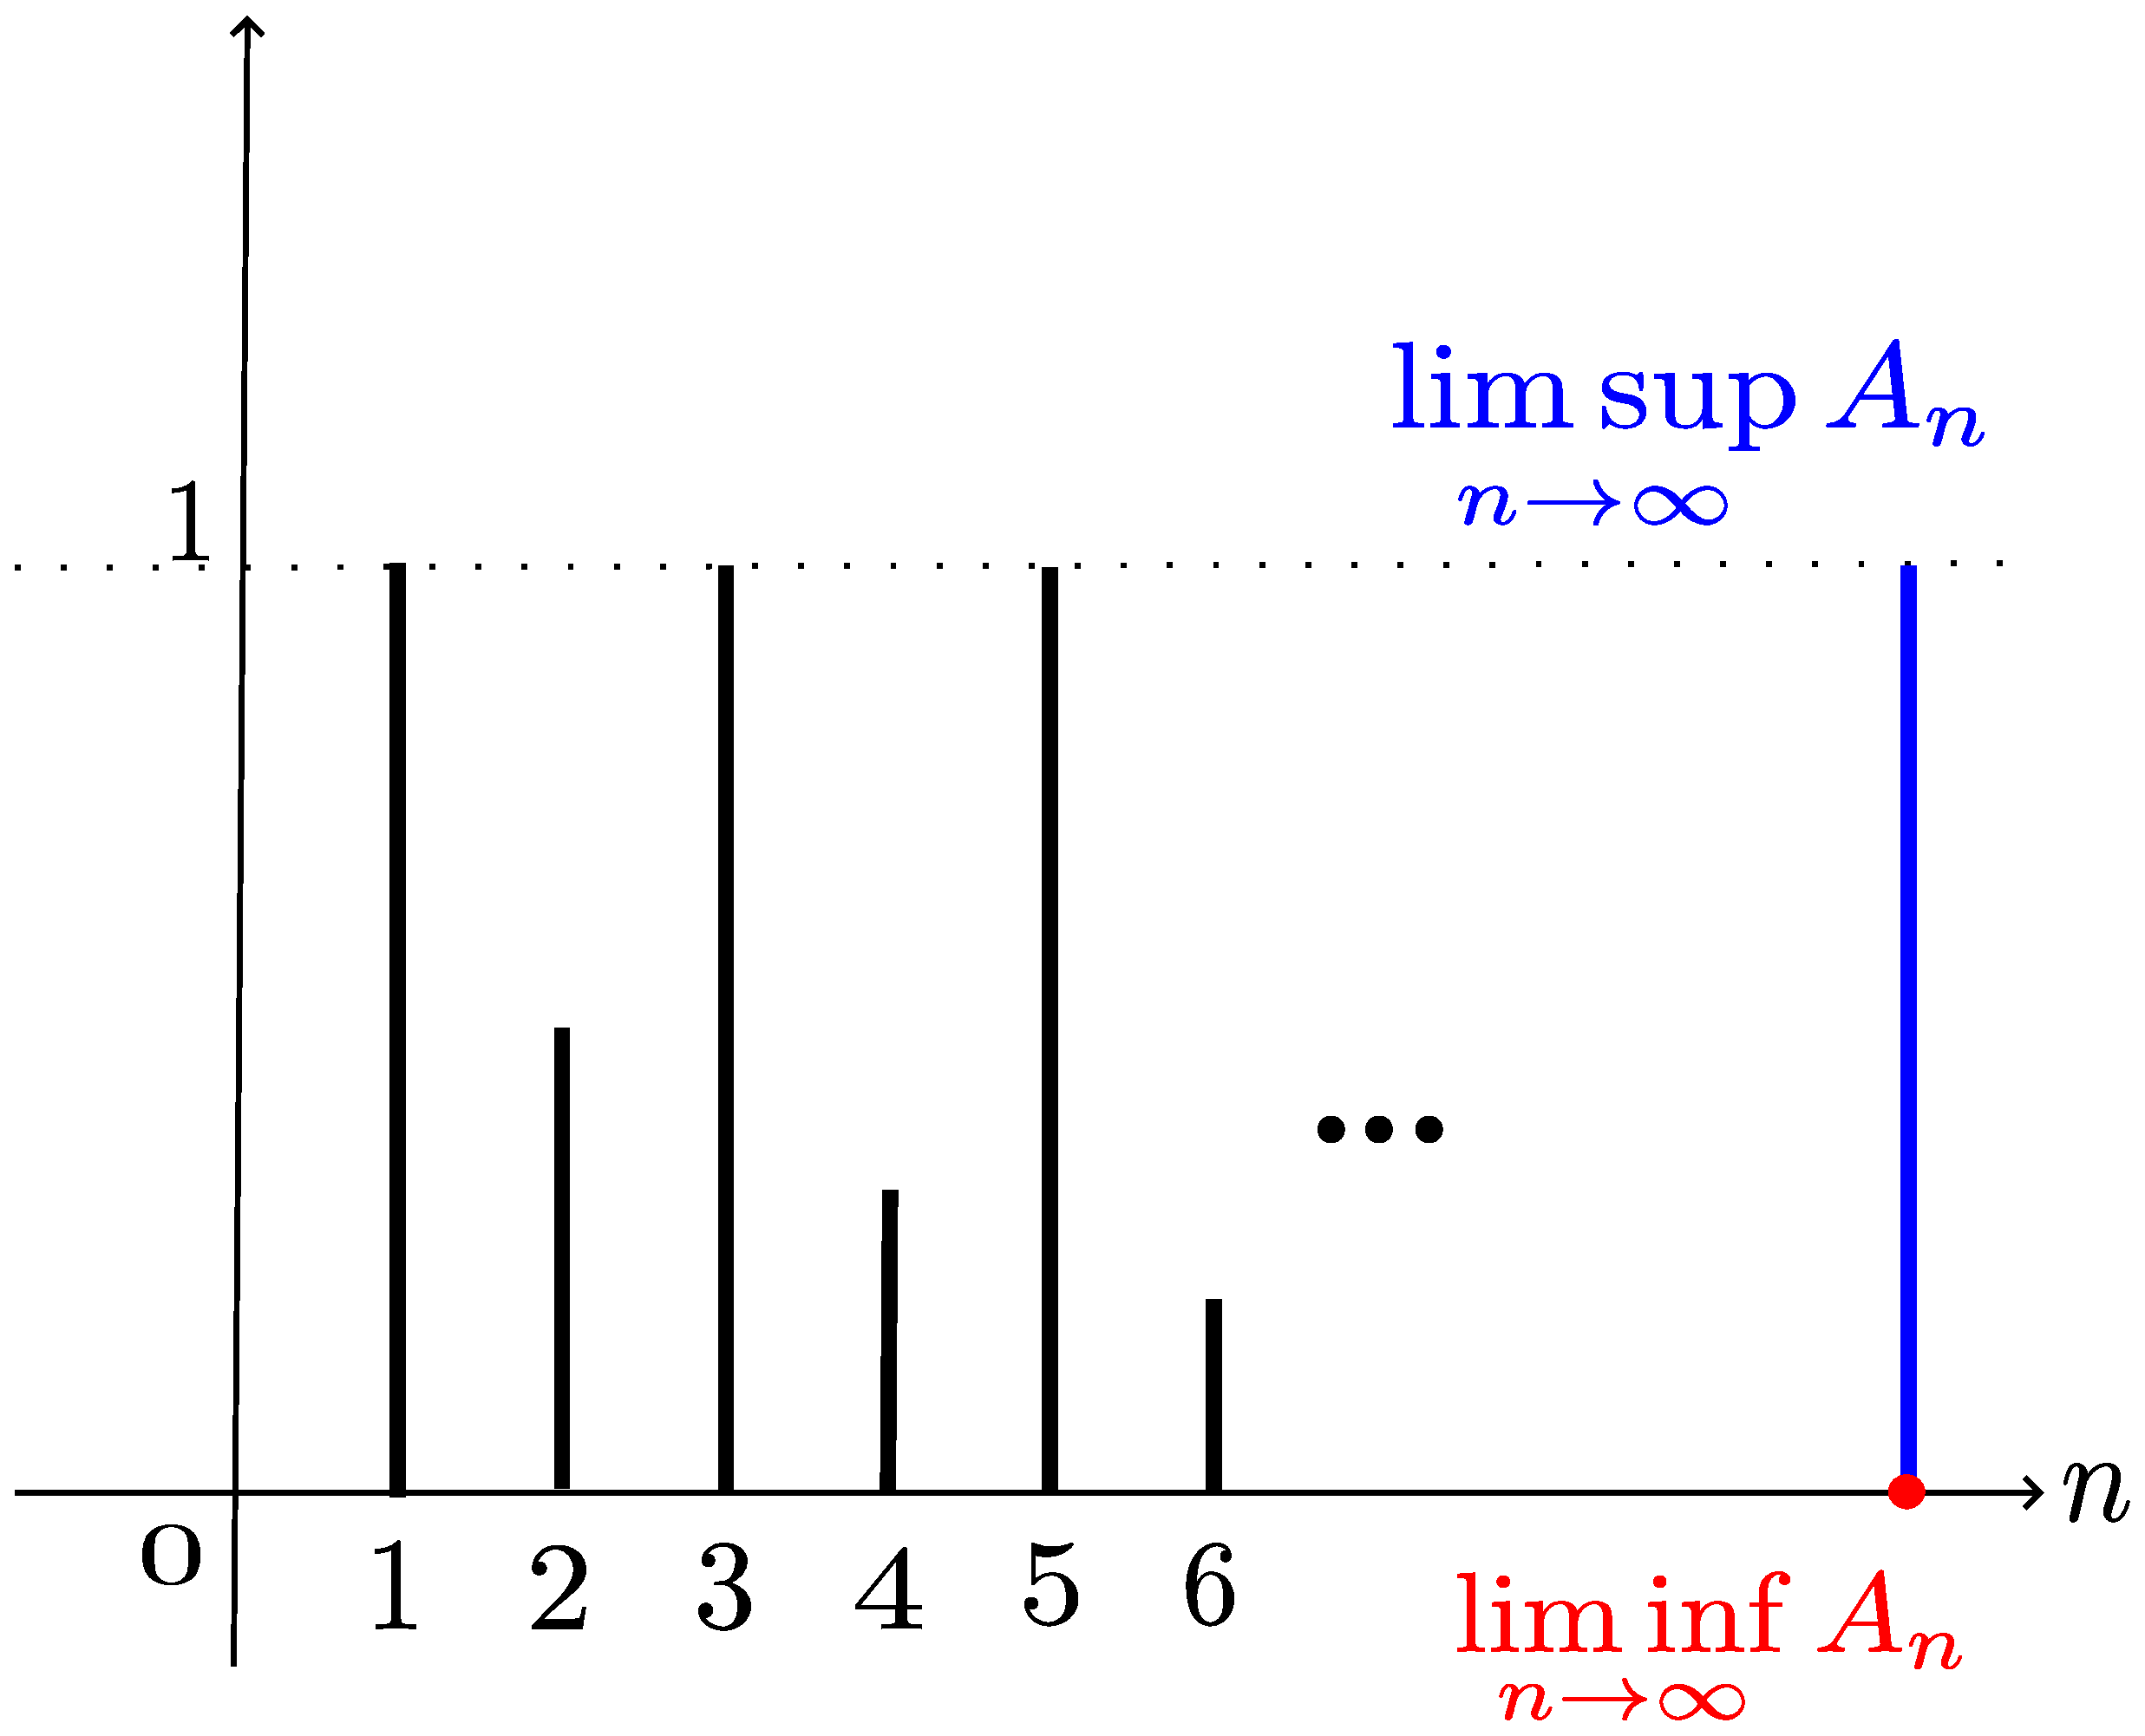
\includegraphics[keepaspectratio, scale=0.160]{figures/example_limsup_and_liminf.eps}
    \end{column}
  \end{columns}
\end{frame}

% 3.3
\begin{frame}[t]{Relations between Asymptotic cones and \Painleve-Kuratowski Convergence}
  \begin{alertblock}{Remark}
    Providing that the given $A_t$ converges in the sense of \Painleve-Kuratowski, we can let $\Gamma (t) = A_t$ and $\Gamma (\infty) = A$ where $A, A_t \subset Y$.
    Then, $\Gamma$ implies a set-valued mapping from $\RealNumberSet_{+}\backslash\{0\}$ to $\mathcal{P}(\NDemenstionalRealEuclidianSpace)$ and it follows that $\Gamma (\infty) = C^1_{\infty} = C_{\infty}$
  \end{alertblock}

  \begin{columns}
    \begin{column}{0.48\textwidth}
    $C$: a nonempty subset in $\NDemenstionalRealEuclidianSpace$ \\
    $\Gamma$: $\RealNumberSet_{+}\backslash\{0\}  \rightarrow \mathcal{P}(\NDemenstionalRealEuclidianSpace)$ \\
    We let $\Gamma (t) = \frac{C}{t}$. \\
    \pause
    \centering
    \begin{equation}
        \begin{split}
            \liminf_{t \to \infty} \frac{C}{t} &= C^1_{\infty} \\
            \limsup_{t \to \infty}\frac{C}{t} &= C_{\infty} \notag
        \end{split}
    \end{equation}
    \end{column}
    \pause
    \begin{column}{0.48\textwidth}
    \centering
    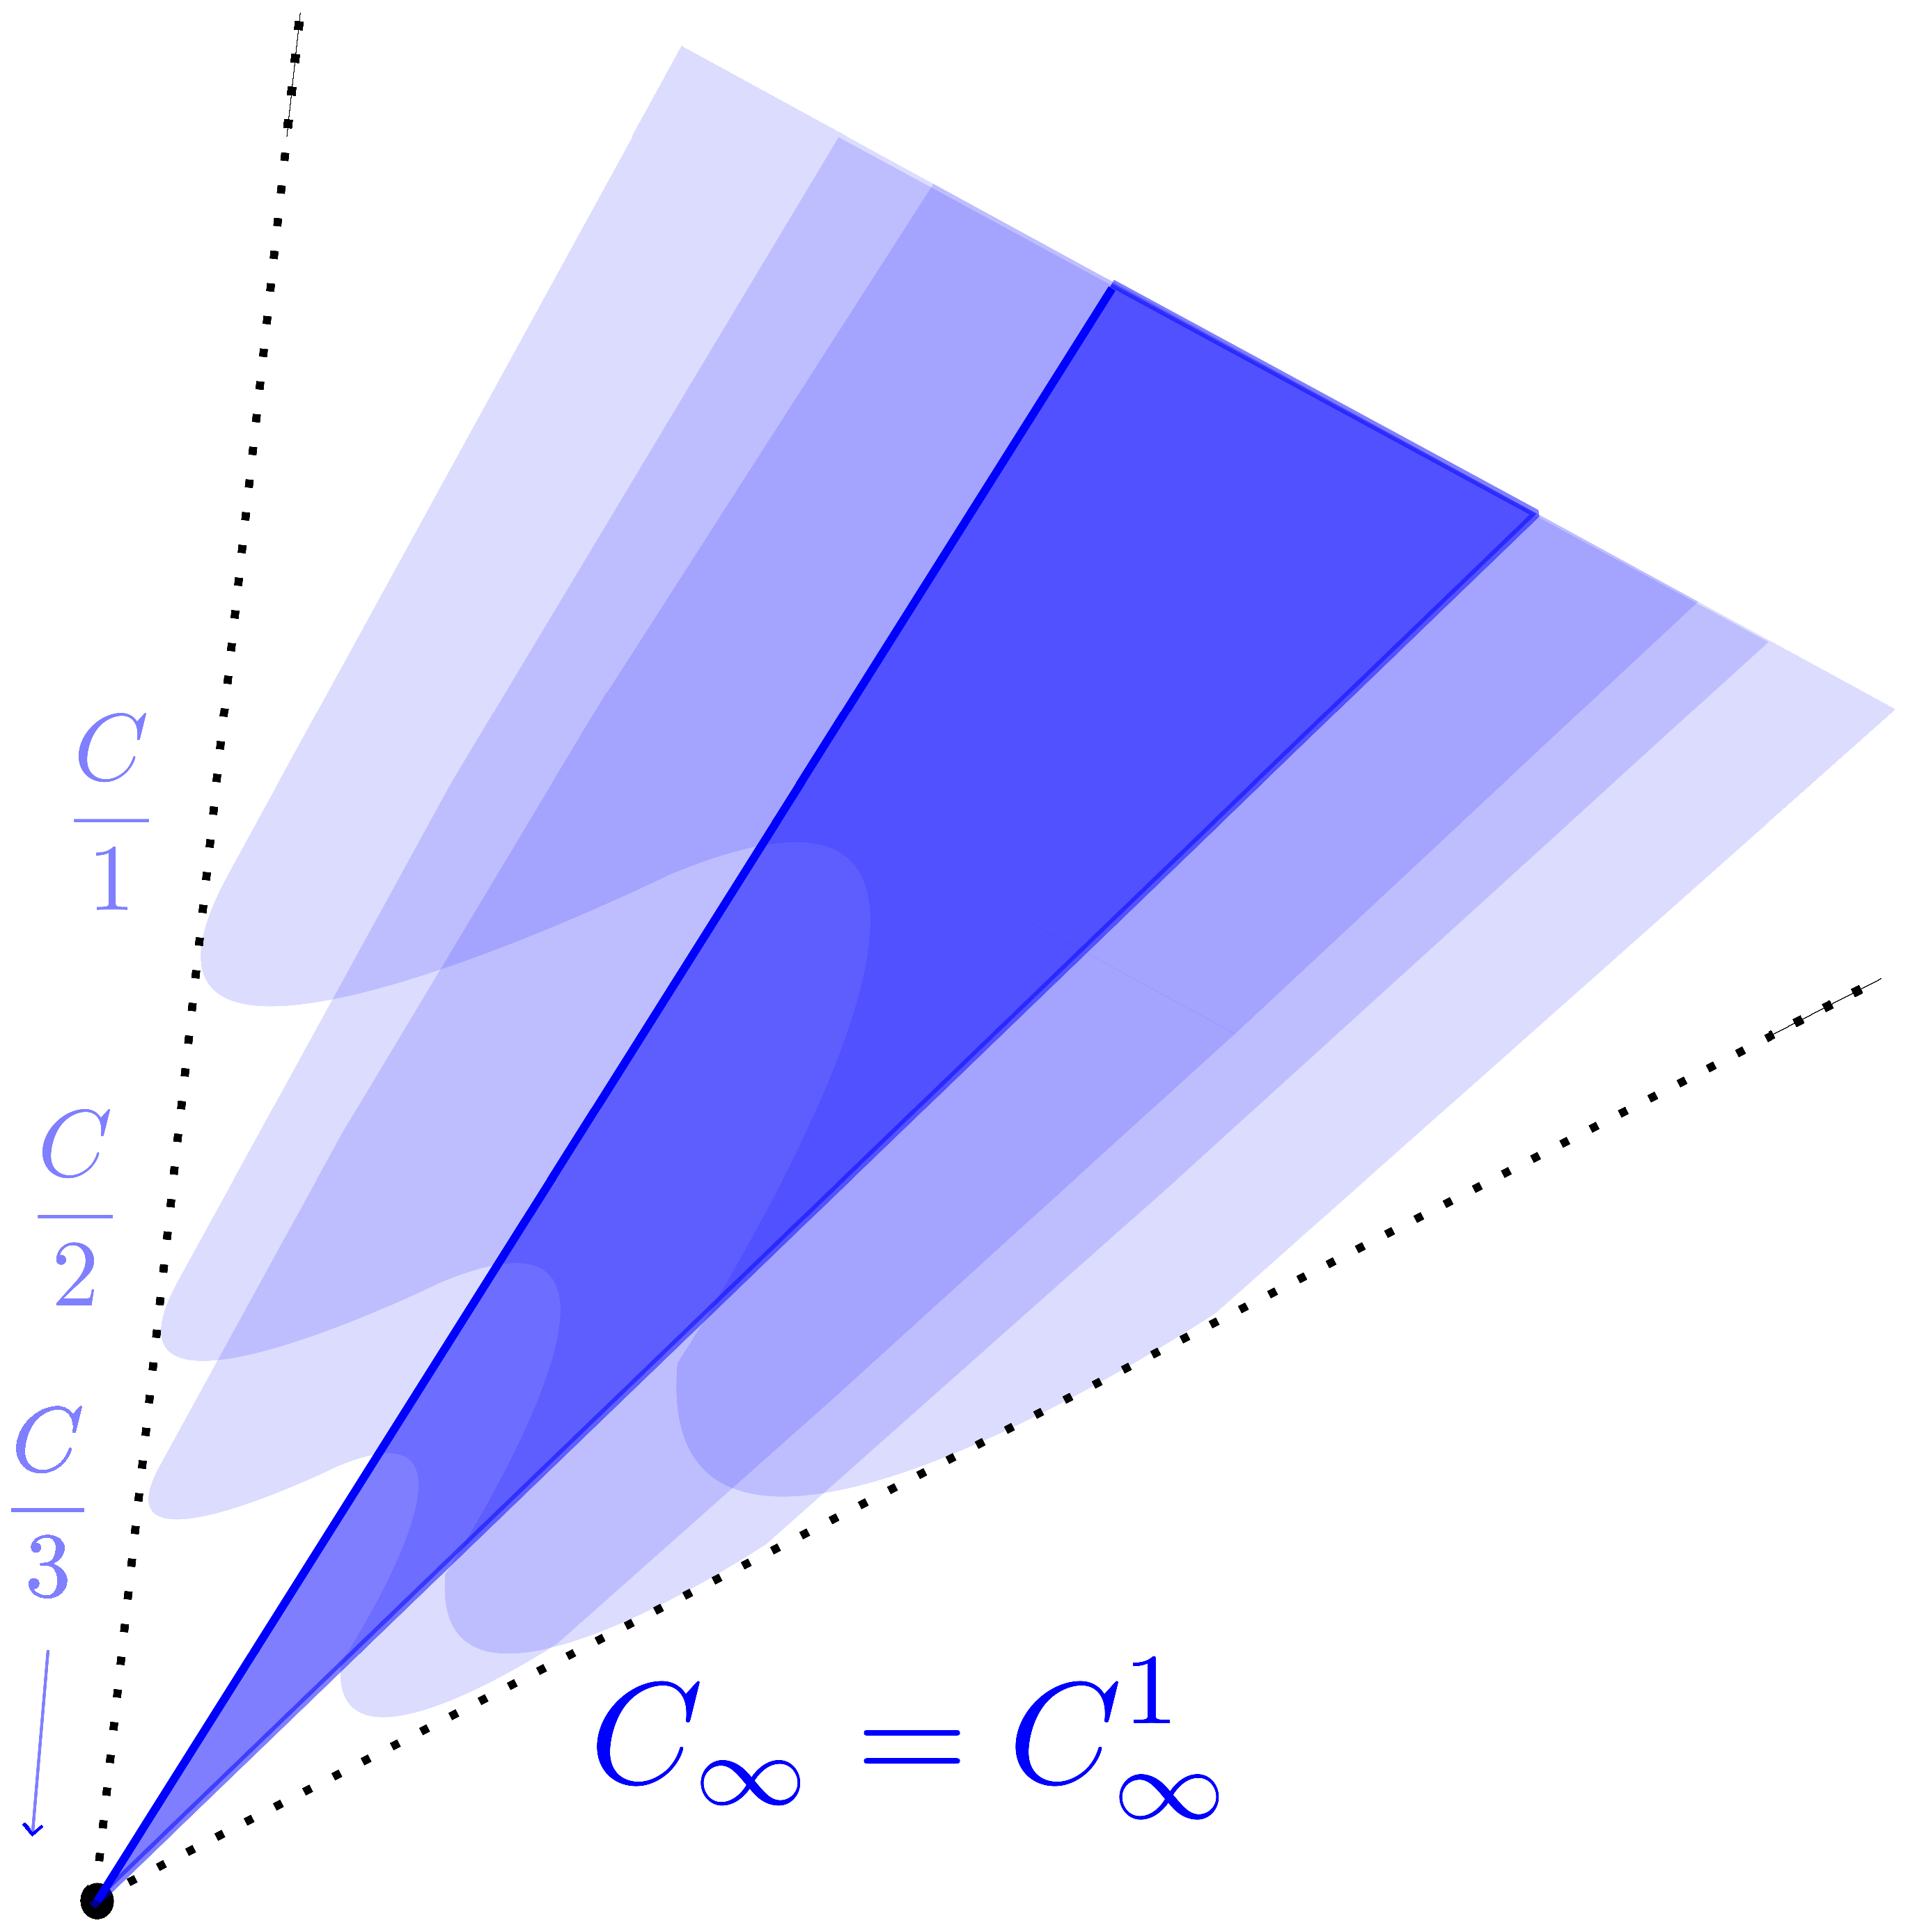
\includegraphics[keepaspectratio, scale=0.09]{figures/relation_asymptotice_cone_and_p_k_convergence.eps}
    \end{column}
  \end{columns}
\end{frame}

% 4.Continuities of set-valued mappings
% ----------------------------------------------------------------
\section{Continuities of set-valued mappings}
\begin{frame}{Contents}
  \tableofcontents[currentsection]
\end{frame}

% 4.1
\begin{frame}[t]{Definition of upper continuity}
  \begin{block}{Definition 4}
    $X, Y$: topological vector spaces, particularly $X$ is a real t.v.s\\
    $\Gamma$: $X \rightarrow \mathcal{P}(Y)$ \\
    $x_0 \in X$ \\
    \medskip
    We say that

    (a) $\Gamma$ is upper continuous (u.c.) at $x_0$ if
    \begin{equation}
      \forall D \subset Y, D \:\text{open}\:, \Gamma (x_0) \subset D, \exists U \in \mathcal{V}_{X}(x_0) \SuchThat \forall x \in U, \Gamma (x) \subset D. \notag
    \end{equation}

    (b) $\Gamma$ is upper continuous (u.c.) if $\Gamma$ is so at every $x_0 \in X$.
  \end{block}
\end{frame}

% 4.2
\begin{frame}[t]{Figure of upper continuity}
  \centering
  \begin{columns}
    \begin{column}{0.48\textwidth}
    \centering
    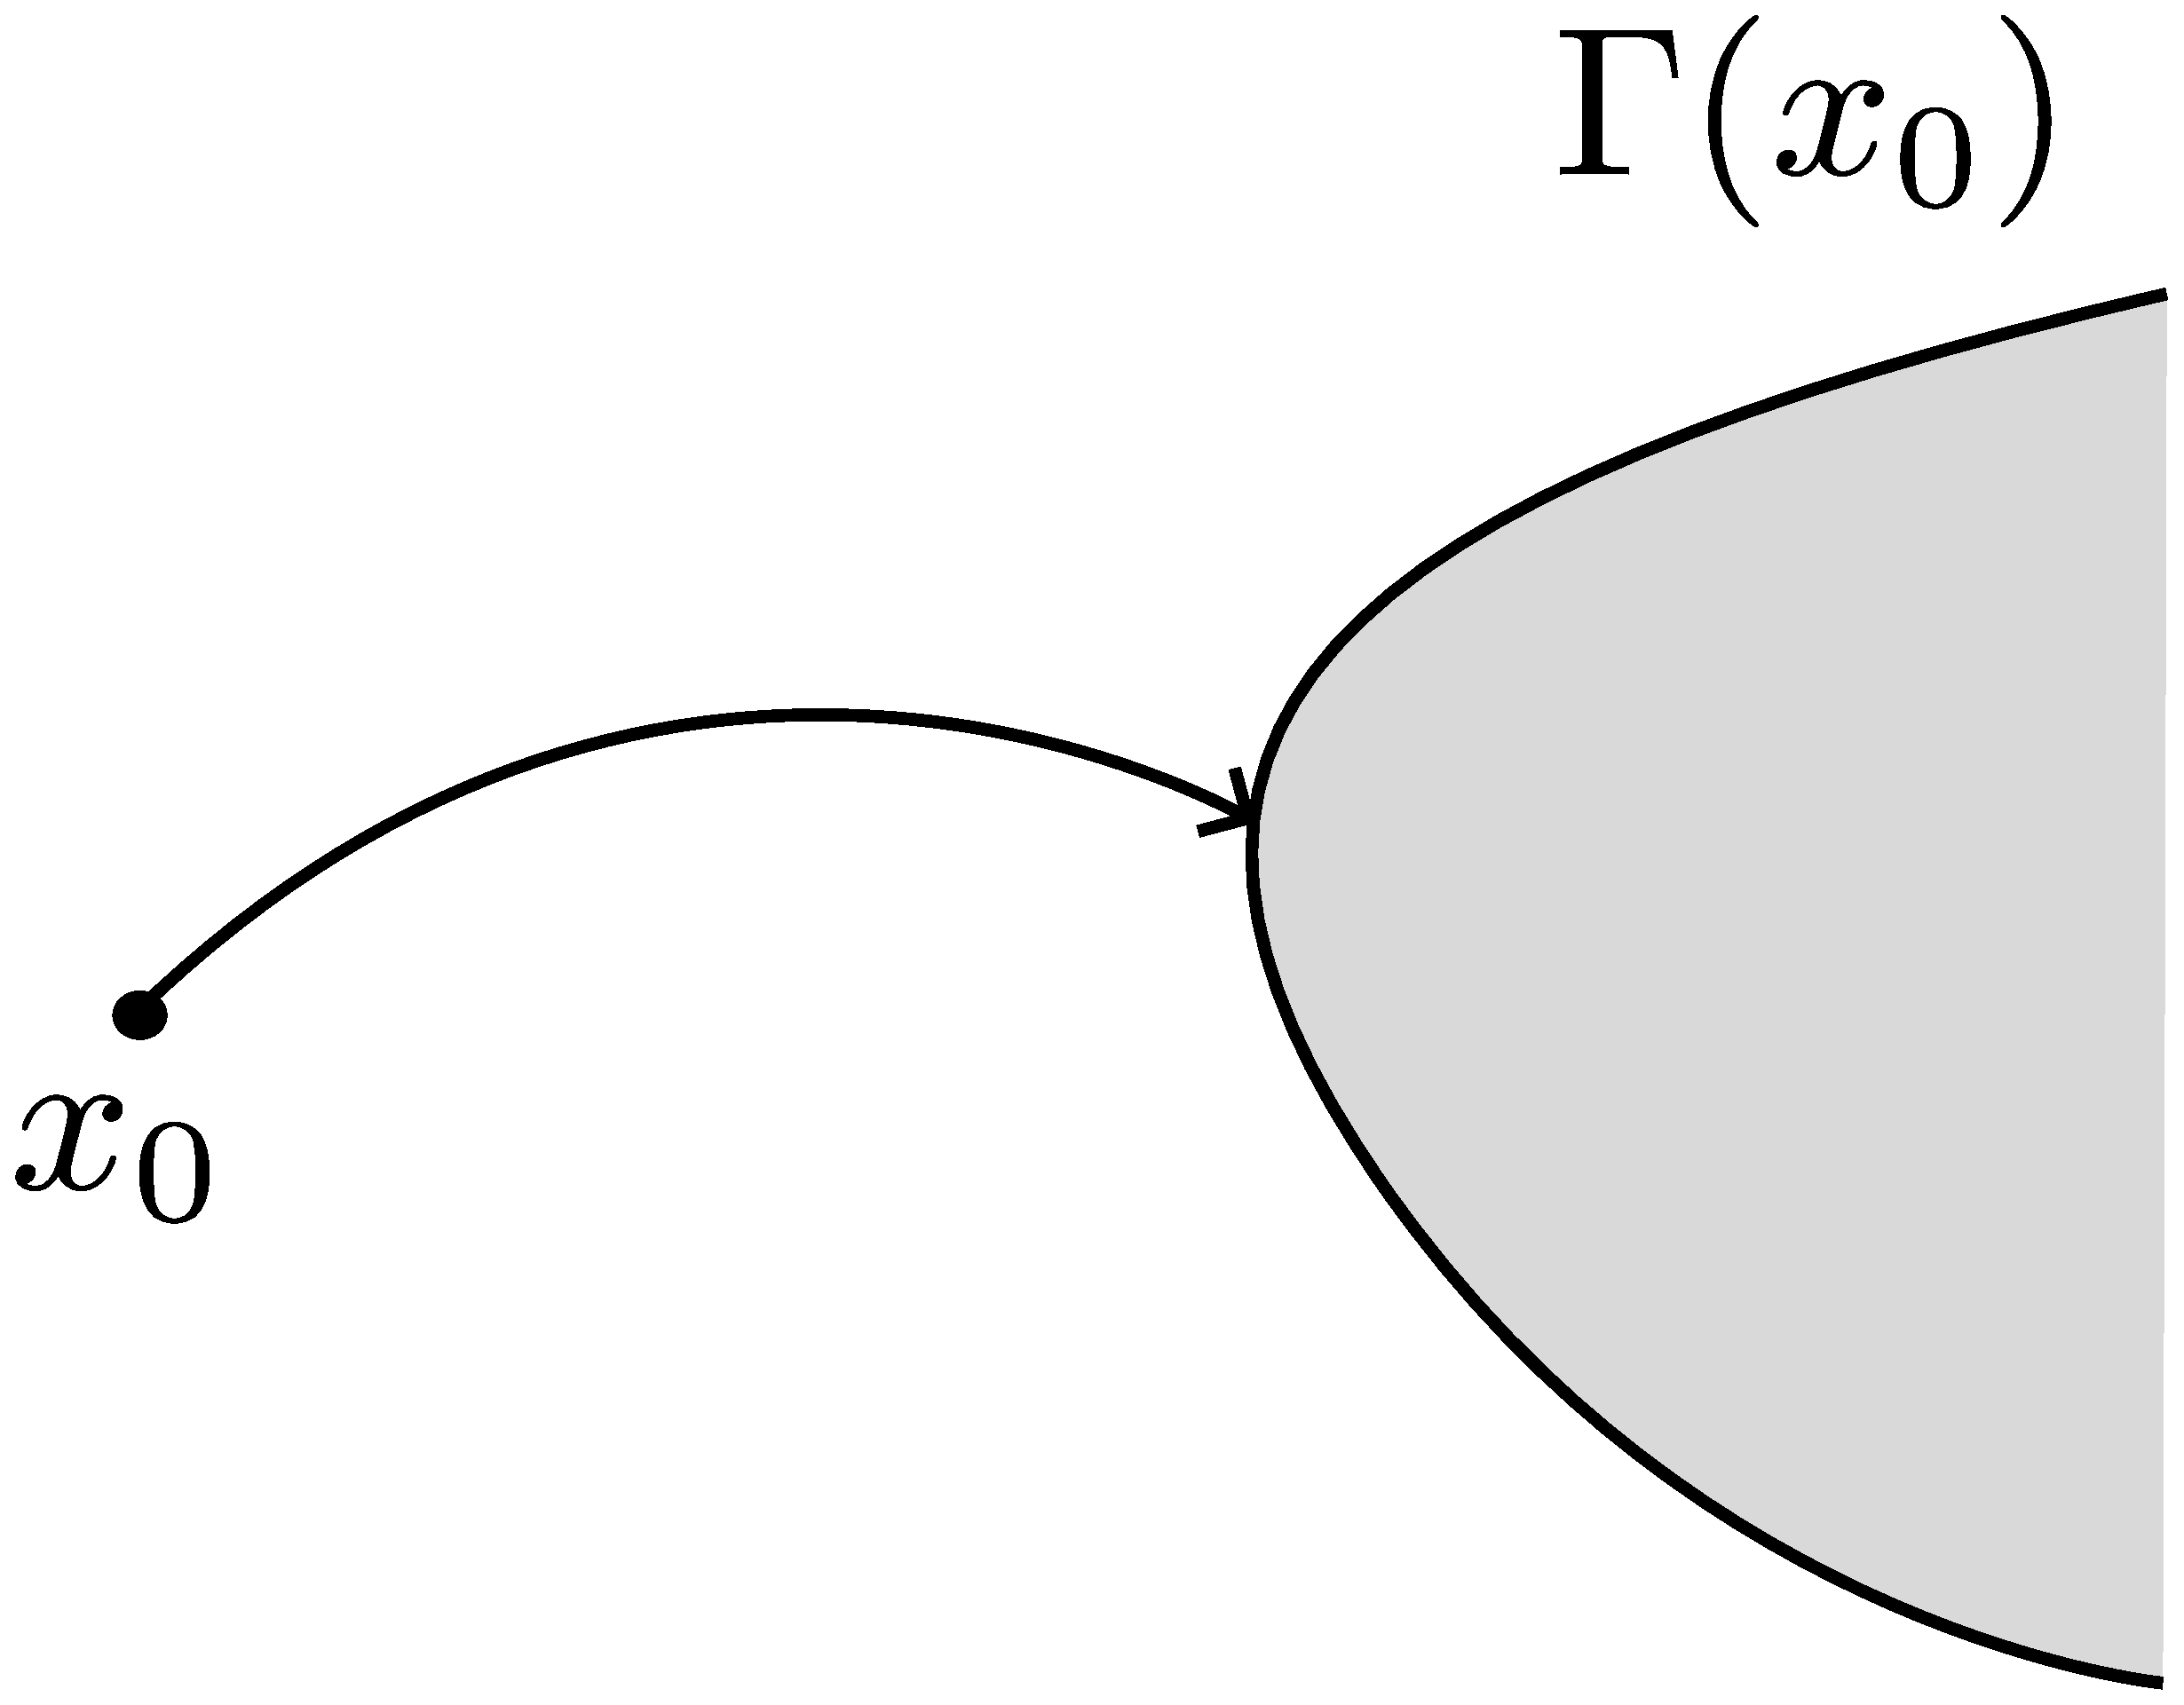
\includegraphics[keepaspectratio, scale=0.16]{figures/continuities/set_valued_mapping.eps}
    \end{column}
    \pause
    \begin{column}{0.48\textwidth}
    \centering
    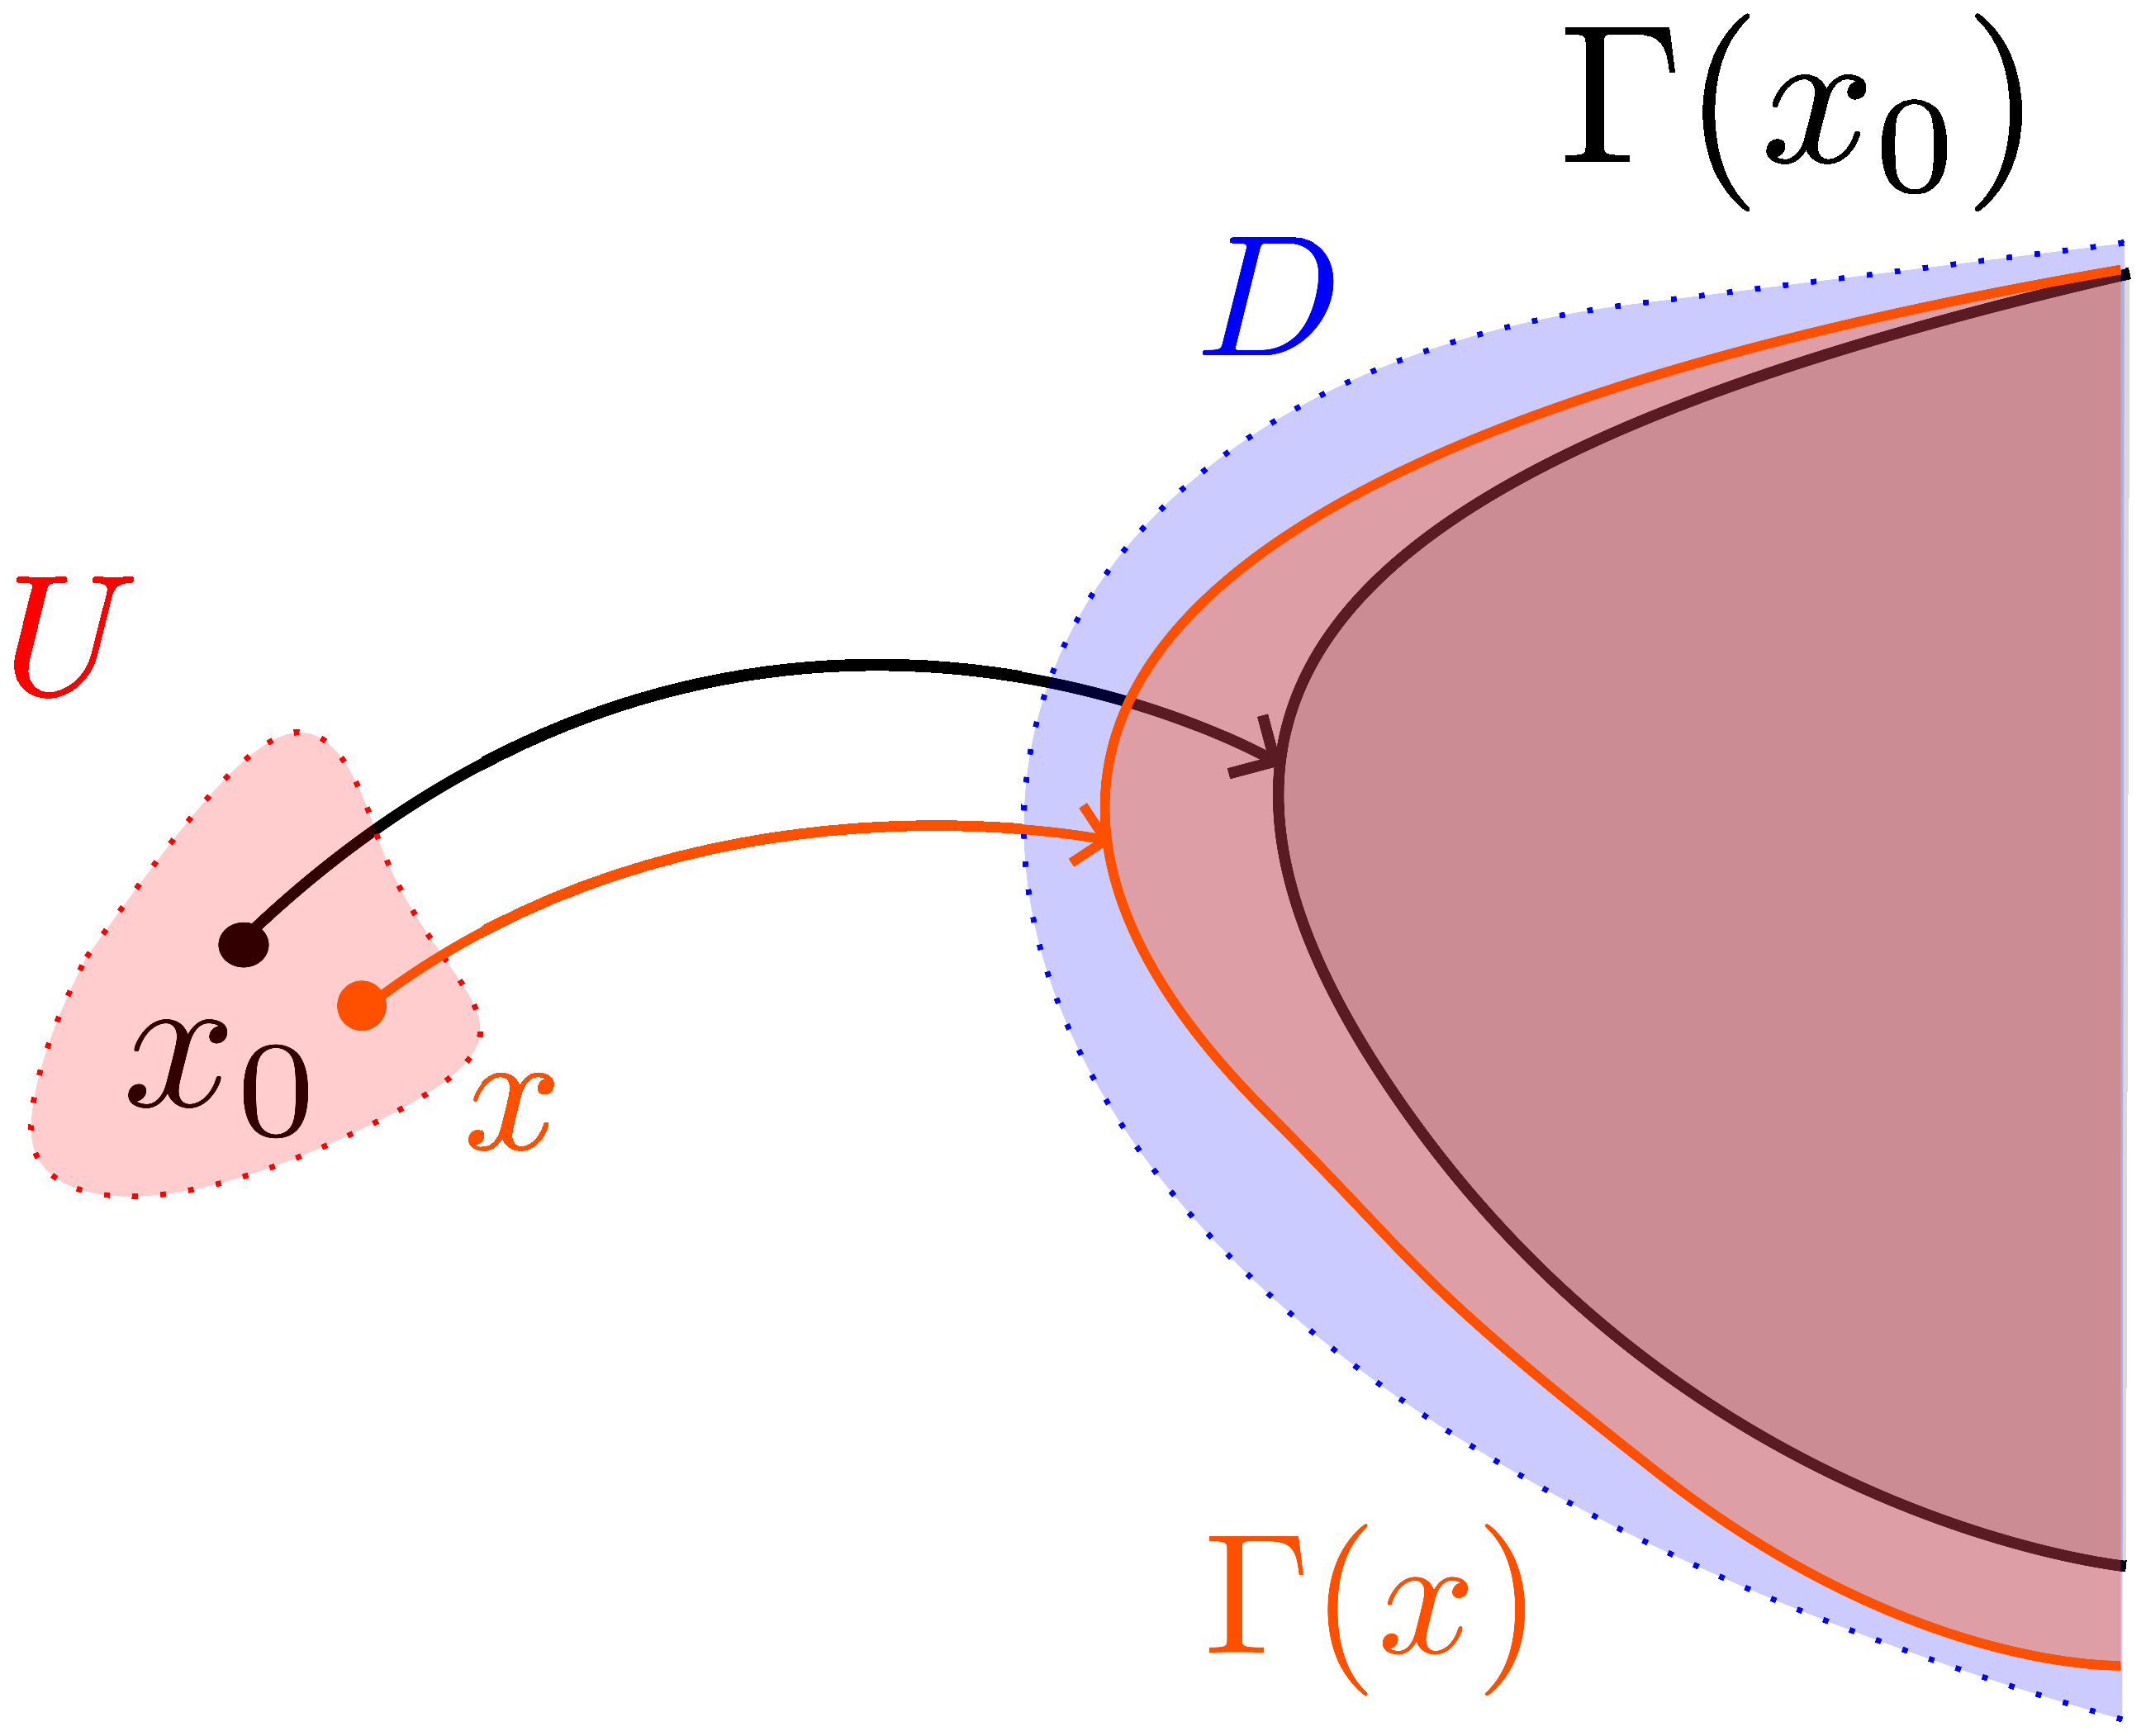
\includegraphics[keepaspectratio, scale=0.16]{figures/continuities/upper_continuity.eps}
    \end{column}
  \end{columns}
\end{frame}

% 4.3
\begin{frame}[t]{Definition of Hausdorff upper continuity}
  \begin{block}{Definition 5}
    $X, Y$: topological vector spaces, particularly $X$ is a real t.v.s\\
    $\Gamma$: $X \rightarrow \mathcal{P}(Y)$ \\
    $x_0 \in X$ \\
    \medskip
    We say that

    (c) $\Gamma$ is Hausdorff upper continuous (H-u.c.) at $x_0$ if
    \begin{equation}
      \forall V \subset \mathcal{V}_Y, \exists U \in \mathcal{V}_{X}(x_0) \SuchThat \forall x \in U, \Gamma (x) \subset \Gamma (x_0) + V. \notag
    \end{equation}

    (d) $\Gamma$ is Hausdorff upper continuous (H-u.c.) if $\Gamma$ is so at every $x_0 \in X$.
  \end{block}
\end{frame}

% 4.4
\begin{frame}[t]{Figure of Hausdorff upper continuity}
  \centering
  \begin{columns}
    \begin{column}{0.48\textwidth}
    \centering
    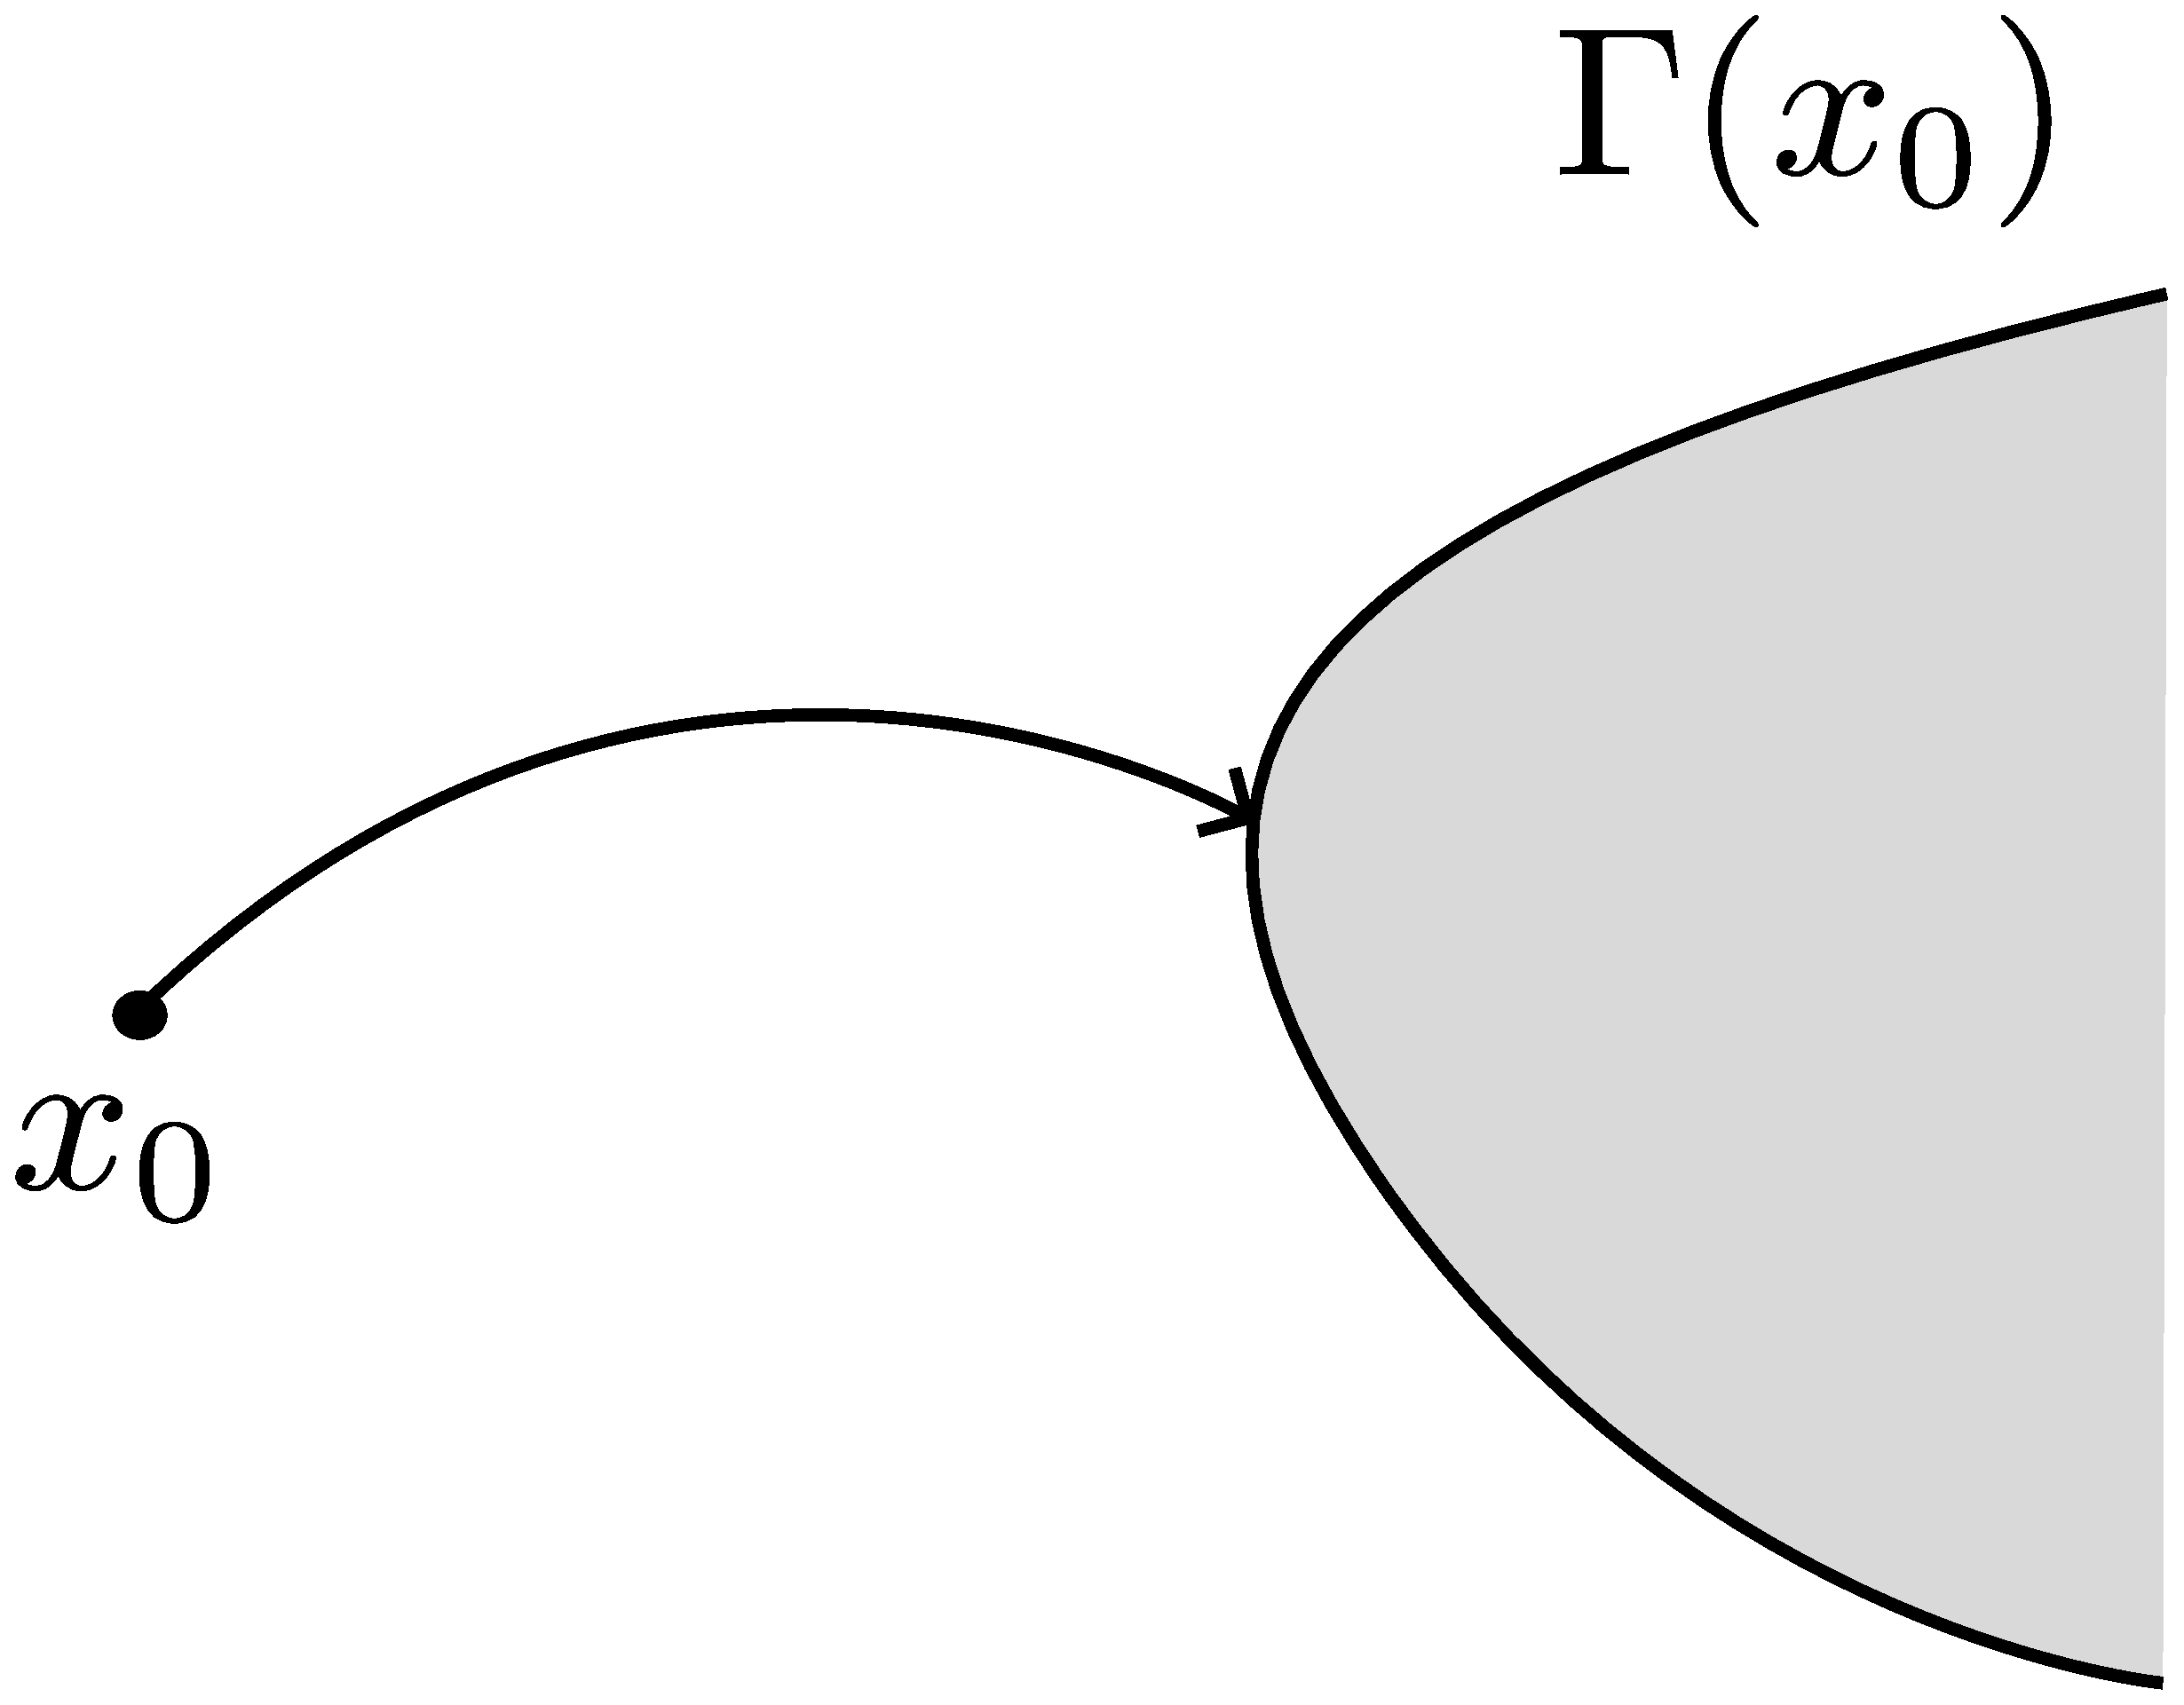
\includegraphics[keepaspectratio, scale=0.16]{figures/continuities/set_valued_mapping.eps}
    \end{column}
    \pause
    \begin{column}{0.48\textwidth}
    \centering
    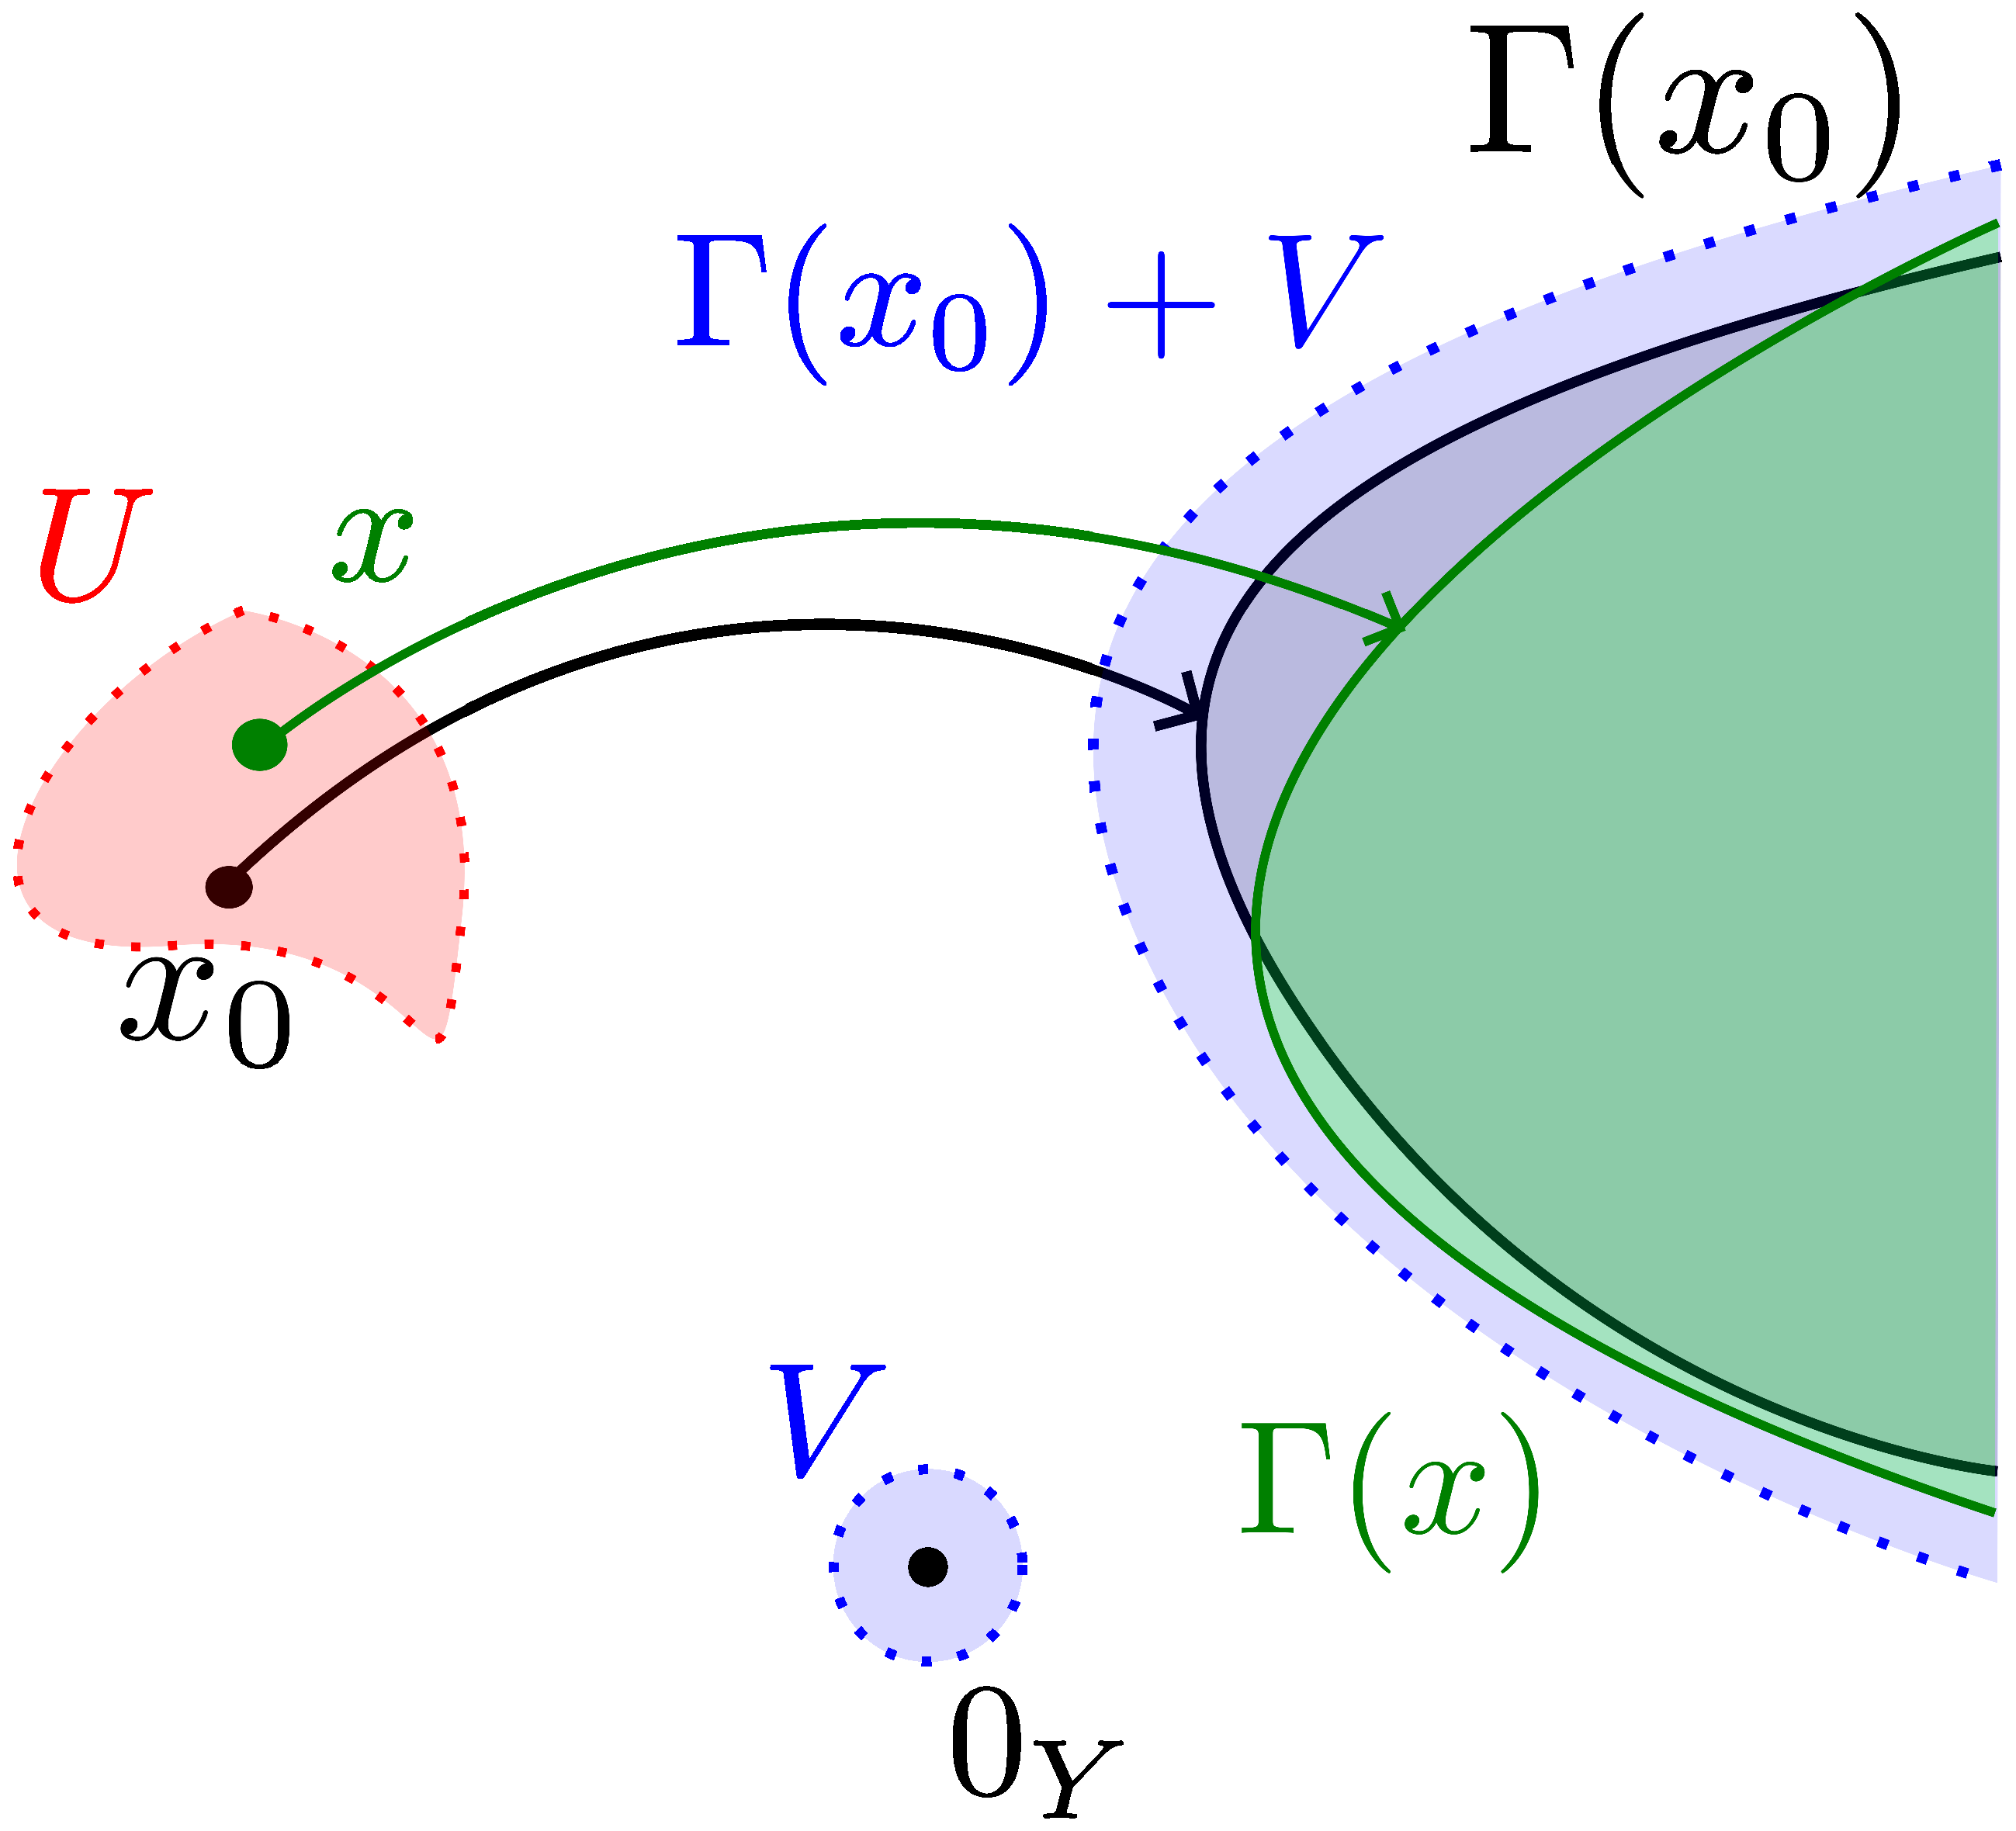
\includegraphics[keepaspectratio, scale=0.16]{figures/continuities/h_upper_continuity.eps}
    \end{column}
  \end{columns}
\end{frame}

% 4.5
\begin{frame}[t]{Relations between Asymptotic cones and these continuities}
  \begin{block}{Relations between Asymptotic cones and these continuities}
    $C$: a nonempty convex subset in $\NDemenstionalRealEuclidianSpace$ \\
    $\Gamma (t) = \frac{C}{t}$ where $t > 0$. \\
    Then, we can see that
    \begin{enumerate}
      \item It does not always hold that $\Gamma$ is upper continuous.
      \item It does not always hold that $\Gamma$ is Hausdorff upper continuous.
    \end{enumerate}
  \end{block}

  \centering
  \begin{columns}
    \pause
    \begin{column}{0.48\textwidth}
    \centering
    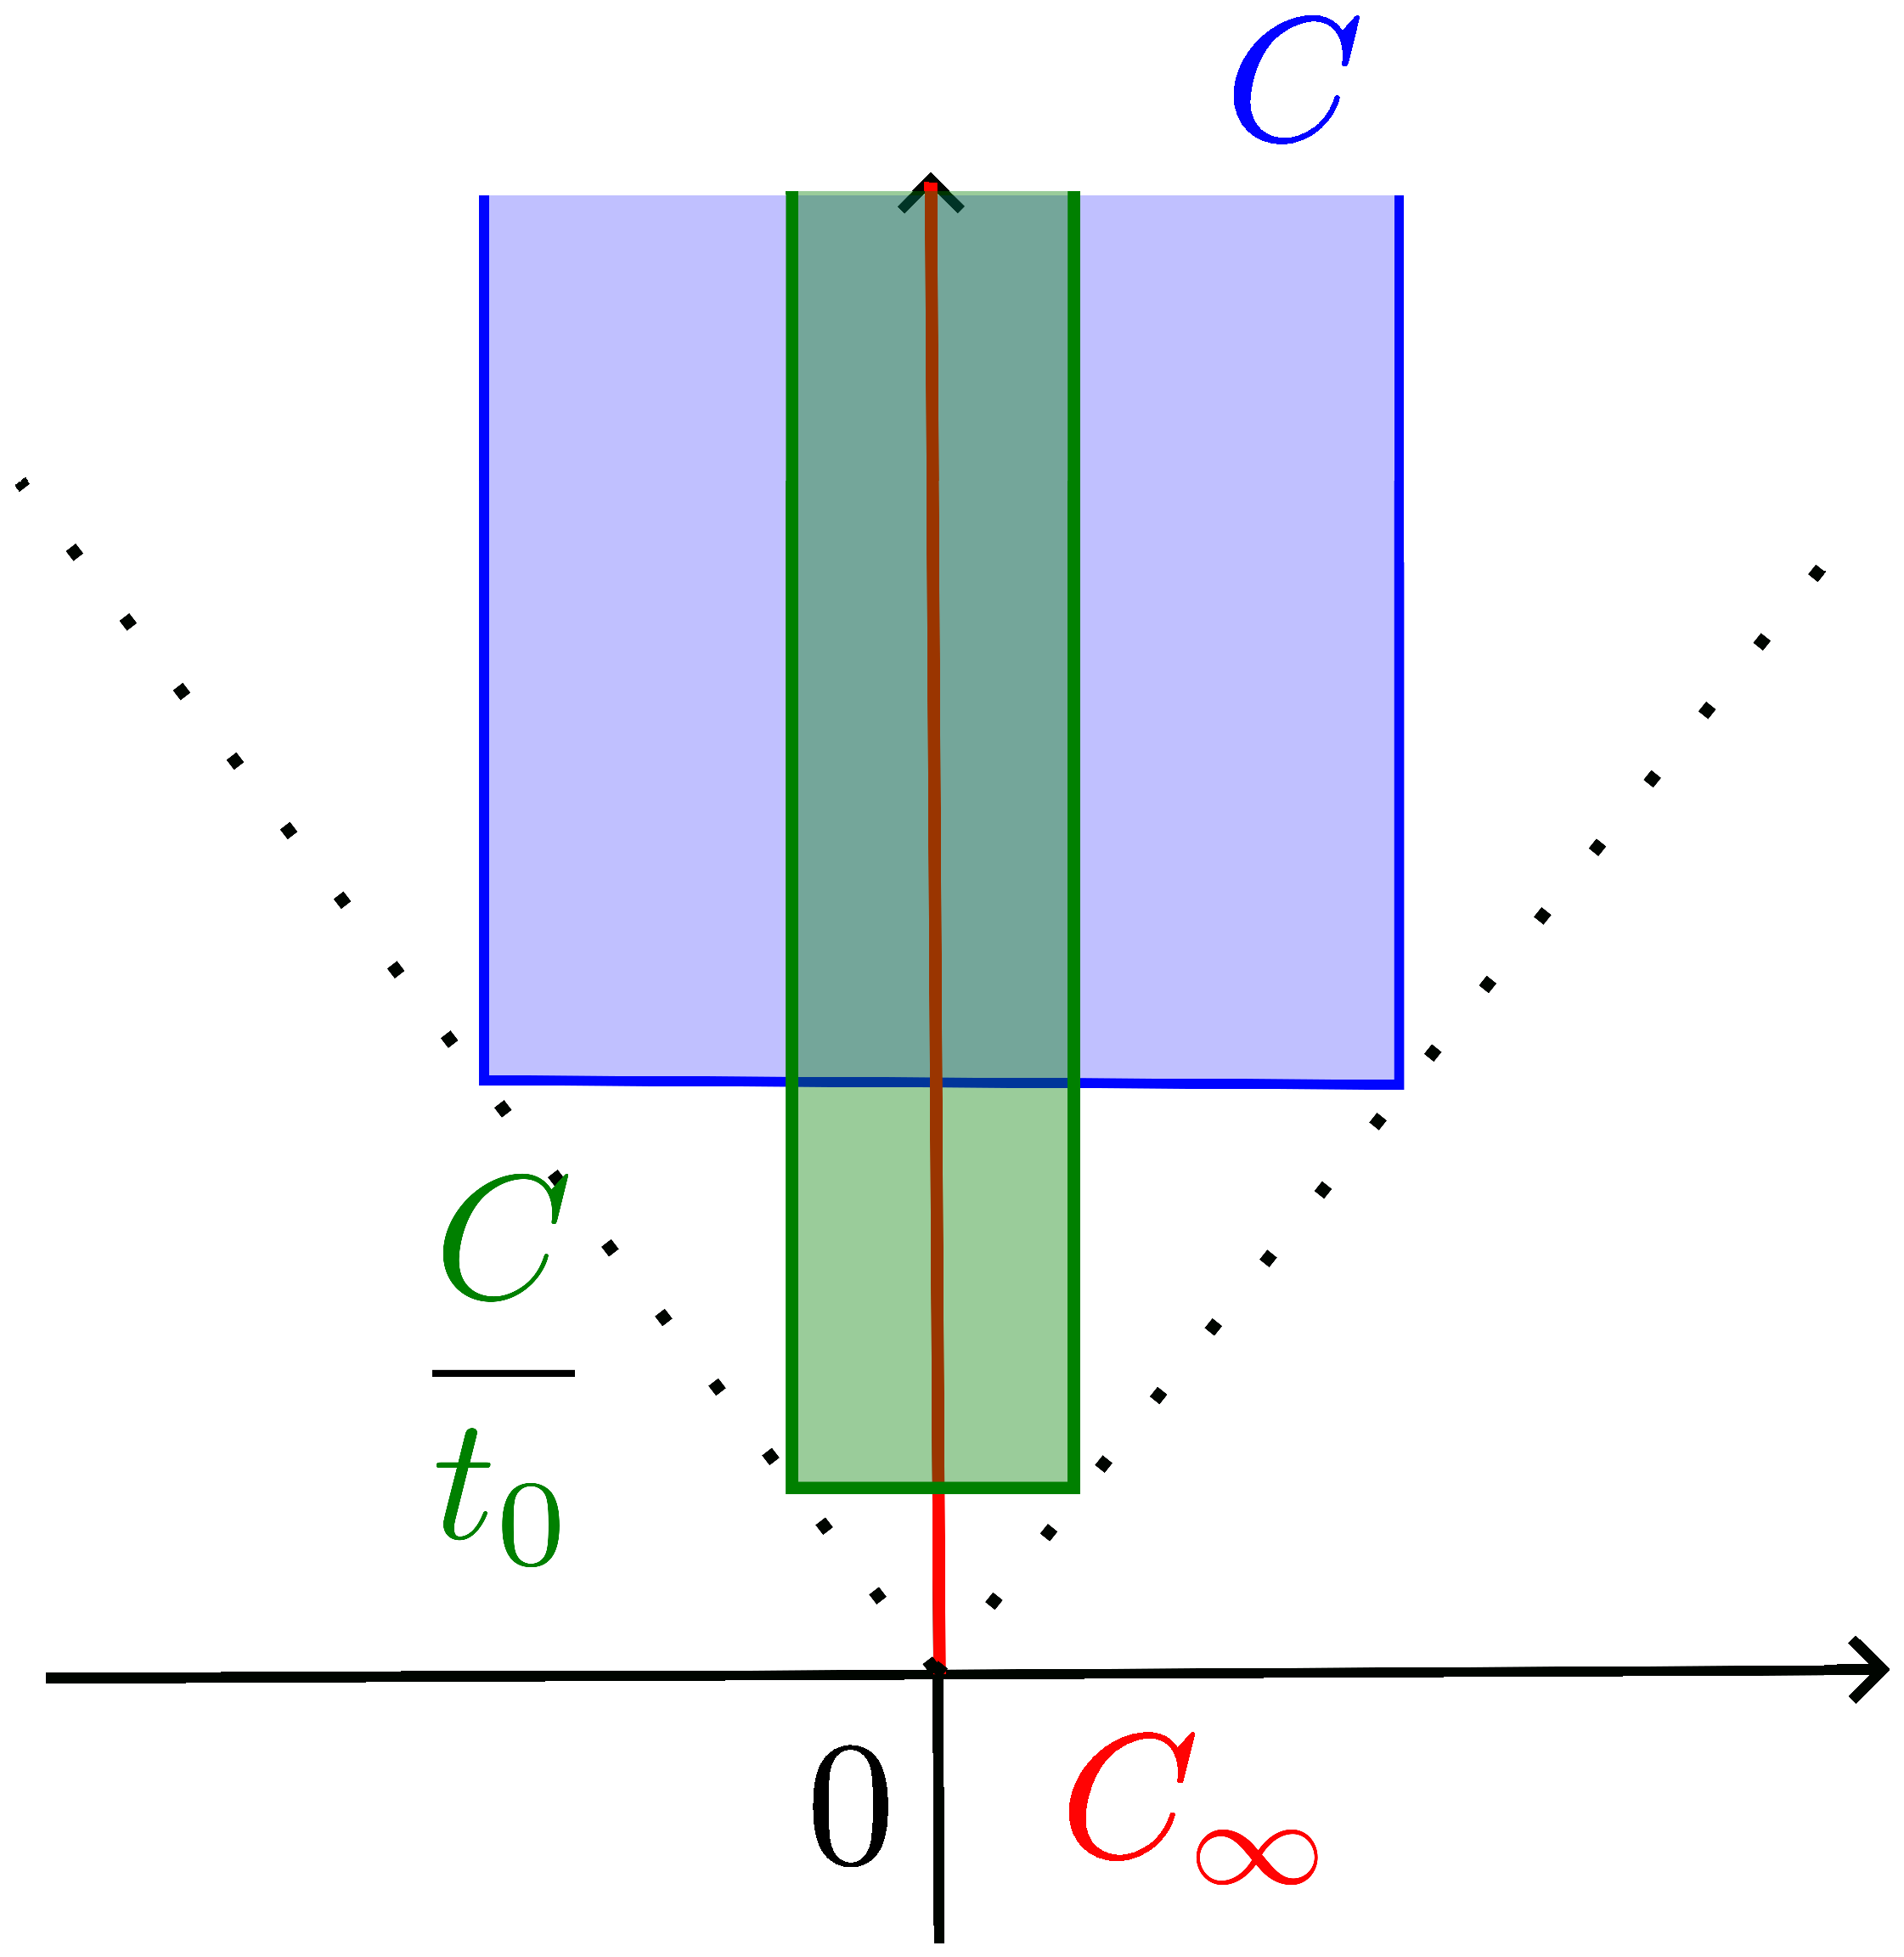
\includegraphics[keepaspectratio, scale=0.085]{figures/continuities/figure_not_uc_but_Huc.eps}
    \end{column}
    \pause
    \begin{column}{0.48\textwidth}
    \centering
    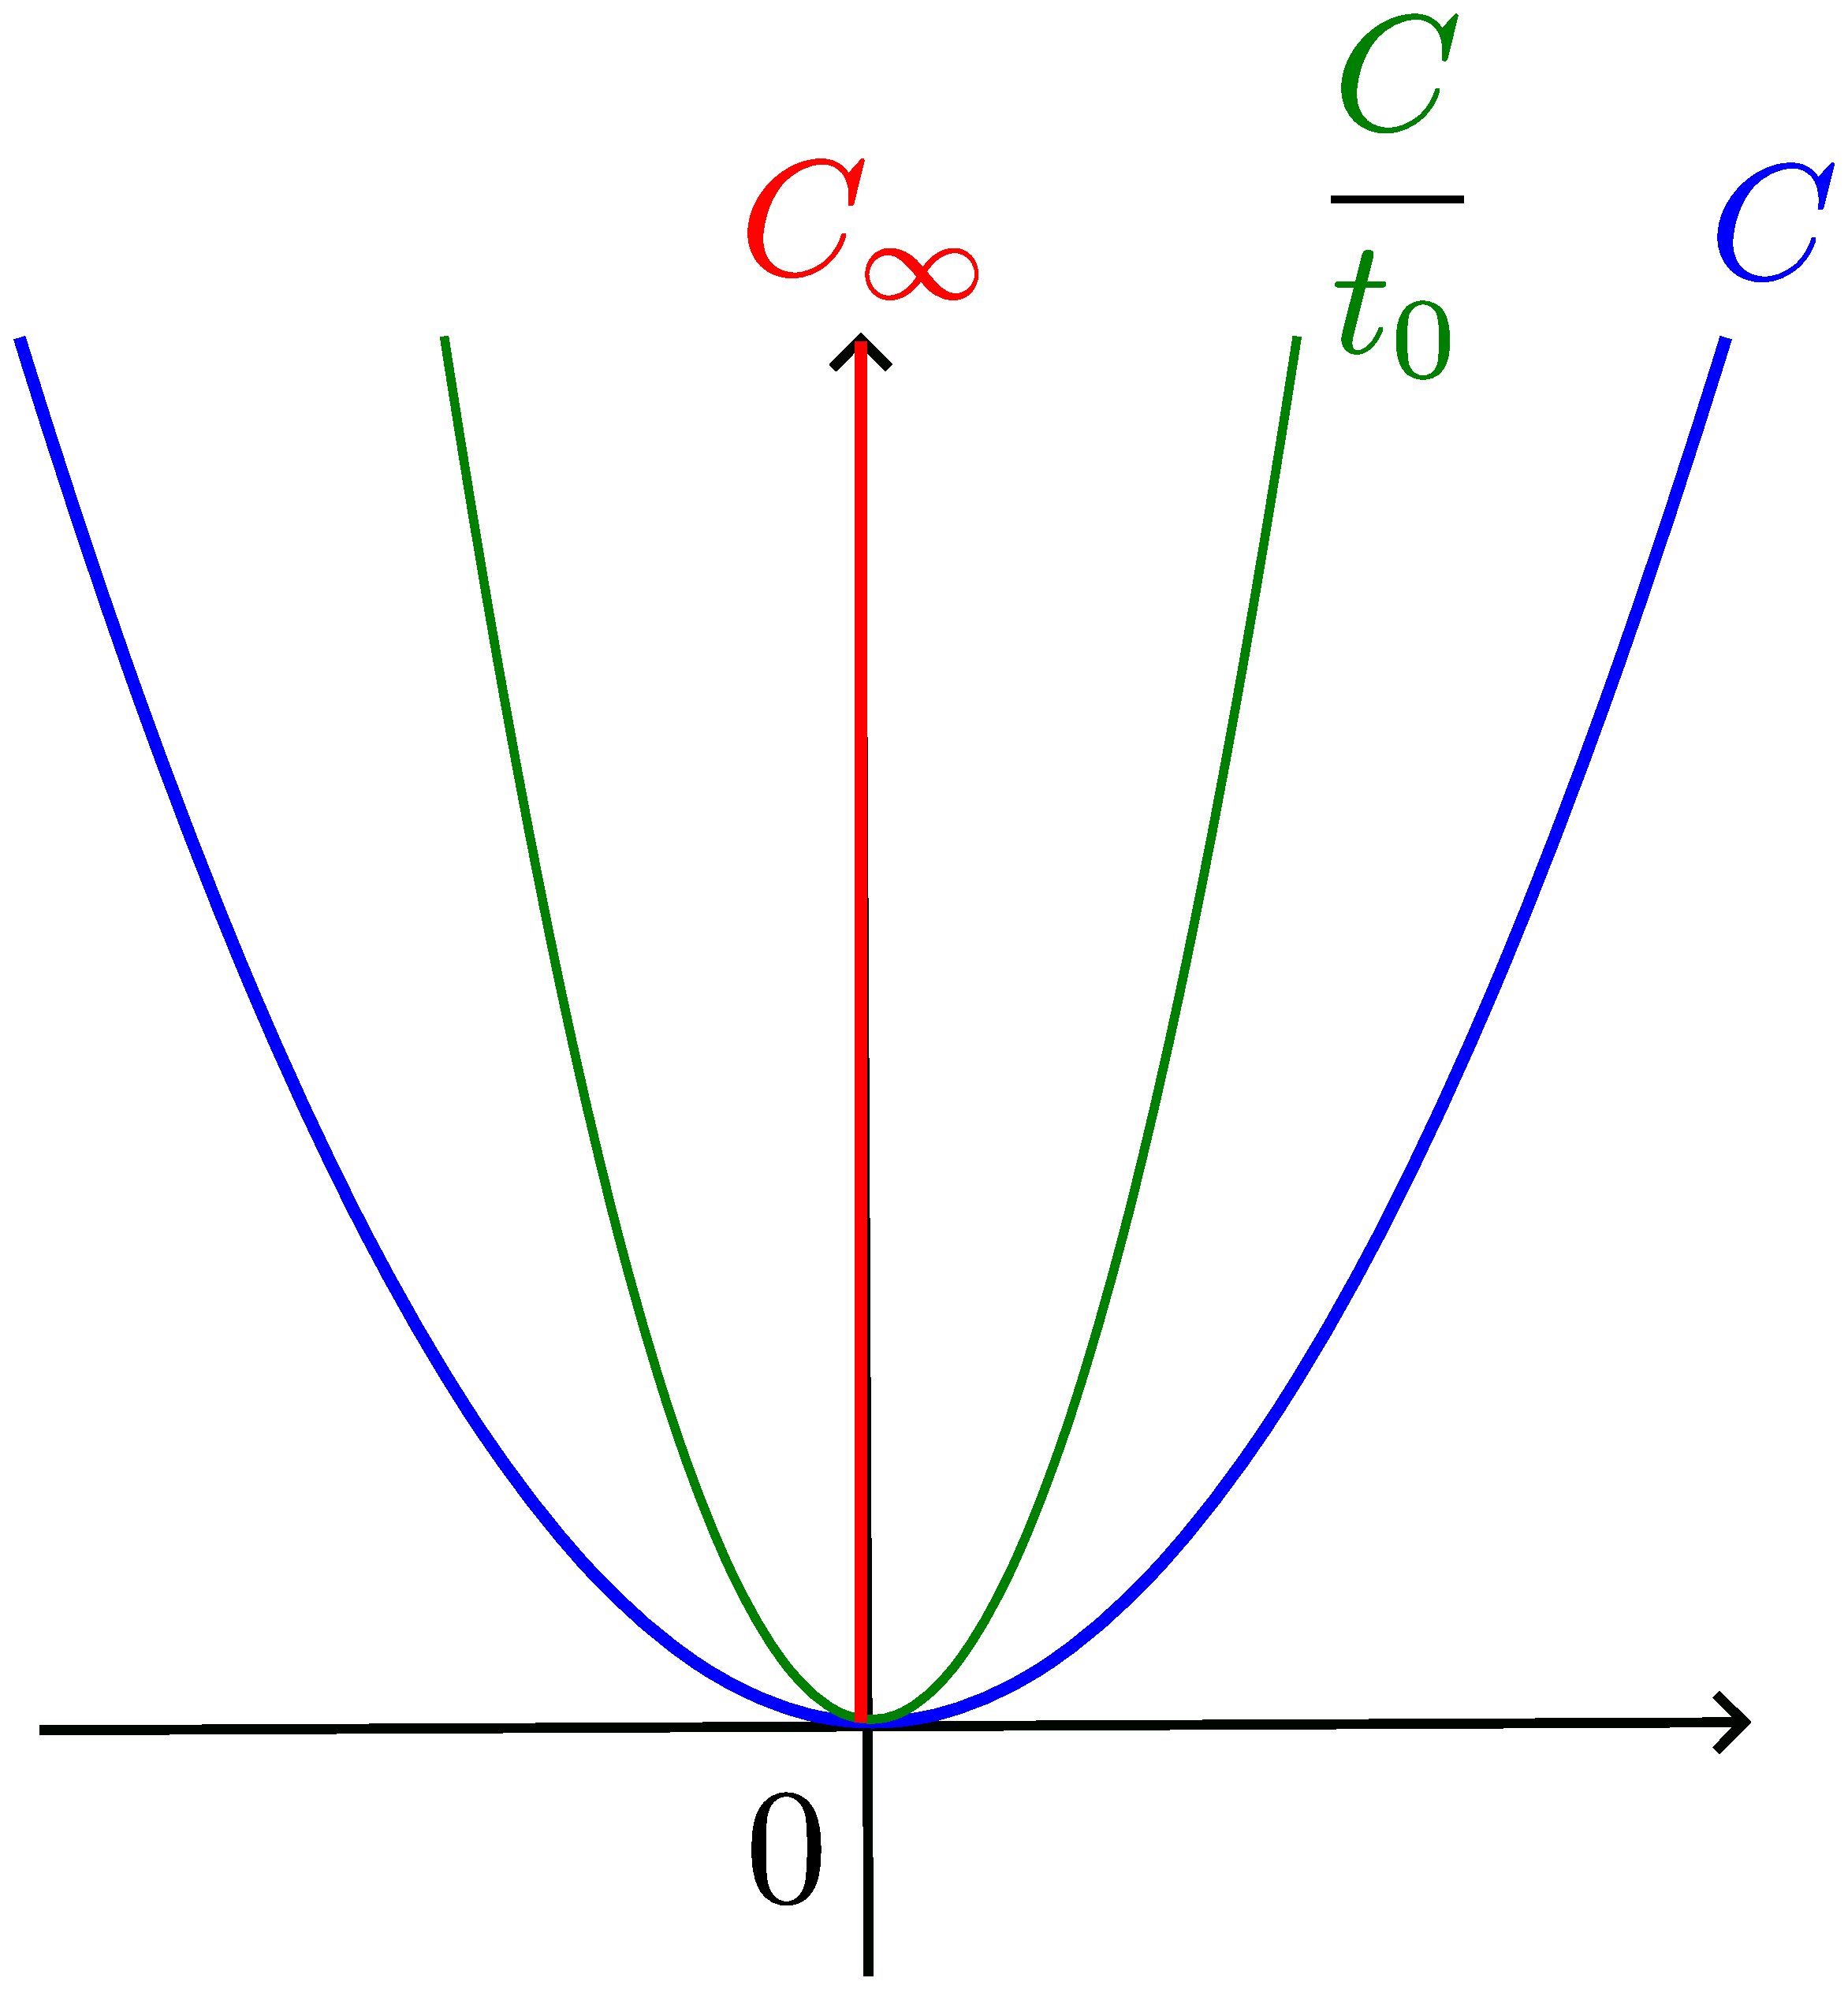
\includegraphics[keepaspectratio, scale=0.082]{figures/continuities/figure_not_uc_and_Huc.eps}
    \end{column}
  \end{columns}
\end{frame}

% 4.6
% \begin{frame}[t]{Generalized cone continuity}
%   \begin{block}{Definition 6}
%     $X, Y$: topological vector spaces
%     $\Gamma$: $X \rightarrow \mathcal{P}(Y)$
%     $x_0 \in X$
%     We say that

%     (a) $\Gamma$ is upper continuous (u.c.) at $x_0$ if
%     \begin{equation}
%       \forall D \subset Y, D \:\text{open}\:, \Gamma (x_0) \subset D, \exists U \in \mathcal{V}_{X}(x_0) \SuchThat \forall x \in U, \Gamma (x) \subset D. \notag
%     \end{equation}

%     (b) $\Gamma$ is upper continuous (u.c.) if $\Gamma$ is so at every $x_0 \in X$.
%   \end{block}
% \end{frame}

% 5.Conclusions
% ----------------------------------------------------------------
\section{Conclusion}
\begin{frame}{Contents}
  \tableofcontents[currentsection]
\end{frame}

% 3.1
\begin{frame}{Conclusion}
  Recap:
  \begin{enumerate}[]
    \item Considering a set-valued mappings, we can replace the definition of asymptotic cones as the outer limit.
    \item Using set-valued mappings allows us to connect the notion of asymptotic cones with some results of continuities in t.v.s.
  \end{enumerate}
  Issues:
  \begin{enumerate}[]
    \item These last results are not enough because we can consider other continuity such as lower continuity.
    \item Particularly, the relation is a case that a given set is convex.
    \item I never combine the relation with applications of asymptotic cones.
  \end{enumerate}

\end{frame}

% 5.References
% ----------------------------------------------------------------
\begin{frame}[t]{References}
  \begin{enumerate}[]
    \item A. Alfred and M. Teboulle, asymptotic cones and functions in optimization and variational inequalities, Springer monographs in Mathematics, Springer-Verlag, New York, 2003.
    \item A. G\"{o}pfert, H. Riahi, C. Tammer, and C. Z\u{a}linescu, Variational methods in partially ordered spaces, vol. 17 of CMS Books in Mathematics, Springer-Verlag, New York, 2003.
  \end{enumerate}
\end{frame}

\end{document}
